\documentclass{whiteboard}
\begin{document}
\begin{frame}[plain,t]
\bbcover{OJ 10099}{The Tourist Guide}{Prof. Edson Alves}{Faculdade UnB Gama}

\end{frame}
\begin{frame}[plain,t]
\vspace*{\fill}

\bbenglish{Mr. G. works as a tourist guide. His current assignment is to take some tourists from one city to another. Some two-way roads connect the cities. For each pair of neighboring cities there is a bus service that runs only between those two cities and uses the road that directly connects them. Each bus service has a limit on the maximum number of passengers it can carry. Mr. G. has a map showing the cities and the roads connecting them. He also has the information regarding each bus service. He understands that it may not always be possible for him to take all the tourists to the destination city in a single trip. For example, consider the following road map of $7$ cities. The edges connecting the cities represent the roads and the number written on each edge indicates the passenger limit of the bus service that runs on that road.}

\vspace*{\fill}
\end{frame}
\begin{frame}[plain,t]
\vspace*{\fill}

\bbtext{O senhor G. trabalha como guia turístico. Sua tarefa atual é levar turistas de uma cidade a outra. As cidades são conectados por algumas estradas de mão dupla. Para cada par de cidades vizinhas há um serviço de ônibus que opera apenas entre estas duas cidades e que utiliza a estrada que as une diretamente. Cada serviço de ônibus tem um limite quanto ao número de passageiros que ele pode transportar. O senhor G. tem um mapa das cidades e das estradas que as conectam. Ele também tem informações a respeito dos serviços de ônibus. Ele entende que nem sempre é possível levar todos os turistas para a cidade de destino em uma única viagem. Por exemplo, considere o seguinte mapa, com $7$ cidades. As arestas conectando as cidades representam as estradas e o número associado a cada aresta indica o limite de passageiros do serviço de ônibus que opera naquela estrada.}

\vspace*{\fill}
\end{frame}
\begin{frame}[plain,t]
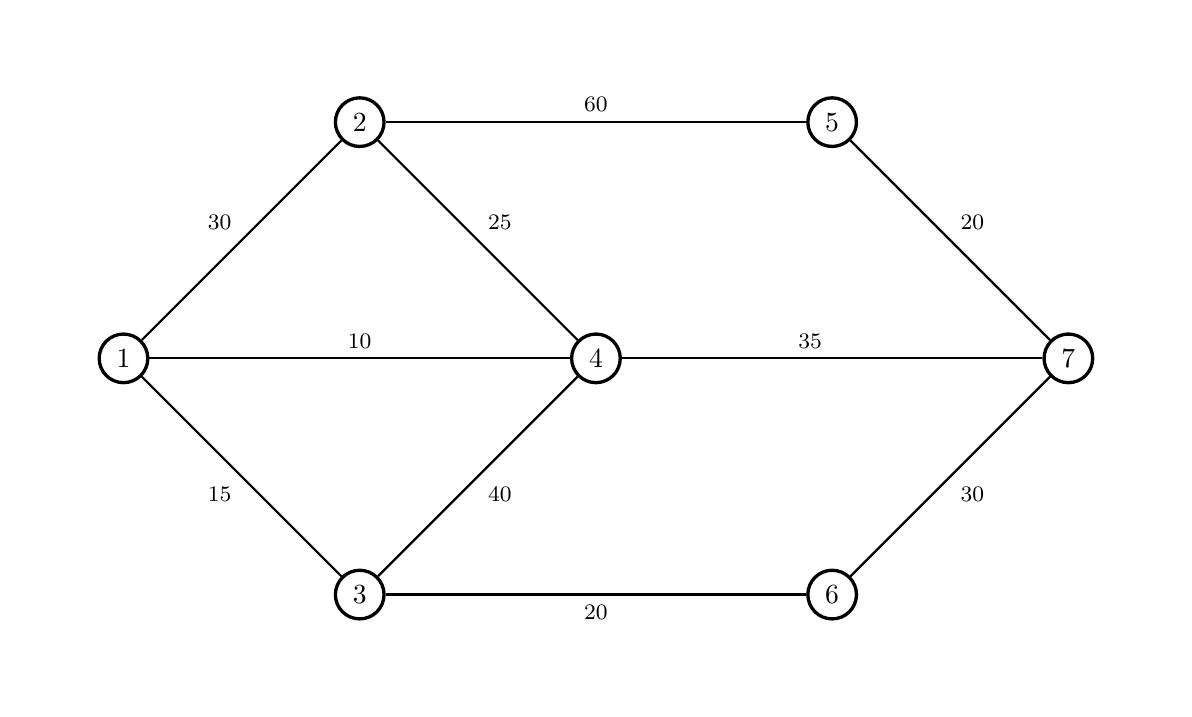
\begin{tikzpicture}
\node[draw,opacity=0] at (0, 0) {x};
\node[draw,opacity=0] at (14, 8) {x};

	\node[draw,circle,very thick] (node1) at (1.0, 4.0) { \bbtext{1} };

	\node[draw,circle,very thick] (node2) at (4.0, 7.0) { \bbtext{2} };

	\node[draw,circle,very thick] (node3) at (4.0, 1.0) { \bbtext{3} };

	\node[draw,circle,very thick] (node4) at (7.0, 4.0) { \bbtext{4} };

	\node[draw,circle,very thick] (node5) at (10.0, 7.0) { \bbtext{5} };

	\node[draw,circle,very thick] (node6) at (10.0, 1.0) { \bbtext{6} };

	\node[draw,circle,very thick] (node7) at (13.0, 4.0) { \bbtext{7} };

	\draw[thick](node1) to node[above left] { \footnotesize \bbinfo{30} } (node2);

	\draw[thick](node1) to node[below left] { \footnotesize \bbinfo{15} } (node3);

	\draw[thick](node1) to node[above] { \footnotesize \bbinfo{10} } (node4);

	\draw[thick](node2) to node[above right] { \footnotesize \bbinfo{25} } (node4);

	\draw[thick](node2) to node[above] { \footnotesize \bbinfo{60} } (node5);

	\draw[thick](node3) to node[below right] { \footnotesize \bbinfo{40} } (node4);

	\draw[thick](node3) to node[below] { \footnotesize \bbinfo{20} } (node6);

	\draw[thick](node4) to node[above left] { \footnotesize \bbinfo{35} } (node7);

	\draw[thick](node5) to node[above right] { \footnotesize \bbinfo{20} } (node7);

	\draw[thick](node6) to node[below right] { \footnotesize \bbinfo{30} } (node7);

\end{tikzpicture}
\end{frame}
\begin{frame}[plain,t]
\vspace*{\fill}

\bbenglish{Now, if he wants to take $99$ tourists from city $1$ to city $7$, he will require at least $5$ trips and the route he should take is : $1$ - $2$ - $4$ - $7$.}

\vspace{0.1in}

\bbenglish{But, Mr. G. finds it difficult to find the best route all by himself so that he may be able to take all the tourists to the destination city in minimum number of trips. So, he seeks your help.}

\vspace*{\fill}
\end{frame}
\begin{frame}[plain,t]
\vspace*{\fill}

\bbtext{Se ele quer levar $99$ turistas da cidade $1$ para a cidade $7$, ele precisará no mínimo de $5$ viagens e a rota que ele deverá seguir é: $1$ - $2$ - $4$ - $7$.}

\vspace{0.1in}

\bbtext{Mas o senhor G. descobriu que é difícil determinar a melhor rota por conta própria, de modo que ele possa levar todos os turistas ao destino deles no menor número de viagens possível. Assim, ele pediu a sua ajuda.}

\vspace*{\fill}
\end{frame}
\begin{frame}[plain,t]
\vspace*{\fill}

\bbbold{Input}

\vspace{0.1in}

\bbenglish{The input will contain one or more test cases. The first line of each test case will contain two integers: $N$ $(N\leq 100)$ and $R$ representing respectively the number of cities and the number of road segments.  Then $R$ lines will follow each containing three integers: $C_1, C_2$ and $P$. $C_1$ and $C_2$ are the city numbers and $P$ $(P > 1)$ is the limit on the maximum number of passengers to be carried by the bus service between the two cities. City numbers are positive integers ranging from $1$ to $N$. The $(R + 1)$-th line will contain three integers: $S, D$ and $T$ representing respectively the starting city, the destination city and the number of tourists to be guided.}

\vspace{0.1in}

\bbenglish{The input will end with two zeroes for $N$ and $R$.}

\vspace*{\fill}
\end{frame}
\begin{frame}[plain,t]
\vspace*{\fill}

\bbbold{Entrada}

\vspace{0.1in}

\bbtext{A entrada é composta por um ou mais casos de teste. A primeira linha de cada caso de teste contém dois inteiros: $N$ $(N\leq 100)$ e $R$, representando o número de cidades e o número de estradas, respectivamente. As $R$ linhas seguintes contém três inteiros: $C_1, C_2$ e $P$. $C_1$ e $C_2$ são os números das cidades e  $P$ $(P > 1)$ é o número máximo de passageiros que podem ser transportados pelo serviço de ônibus entre as duas cidades. Os números das cidades são inteiros postiviso entre $1$ e $N$. A $(R + 1)$-ésima linha contém três inteiros: $S, D$ e $T$, representando o ponto de partida, o destino e o número de turistas a serem guiados, respectivamente.}

\vspace{0.1in}

\bbtext{A entrada termina com dois zeros para $N$ e $R$.}

\vspace*{\fill}
\end{frame}
\begin{frame}[plain,t]
\vspace*{\fill}

\bbbold{Output}

\vspace{0.1in}

\bbtext{For each test case in the input first output the scenario number. Then output the minimum number of trips required for this case on a separate line. Print a blank line after the output of each test case.}

\vspace*{\fill}
\end{frame}
\begin{frame}[plain,t]
\vspace*{\fill}

\bbbold{Saída}

\vspace{0.1in}

\bbtext{Para cada caso de teste da entrada imprima o número do cenário. Entãoa imprima o número mínimo de viagens necessárias neste caso em uma linha. Imprima uma linha em branco após a saída de cada caso de teste.}

\vspace*{\fill}
\end{frame}
\begin{frame}[plain,t]
\begin{tikzpicture}
\node[draw,opacity=0] at (0, 0) {x};
\node[draw,opacity=0] at (14, 8) {x};

	\node[anchor=west] (header) at (0, 7.0) { \bbbold{Exemplo de entrada e saída} };

\end{tikzpicture}
\end{frame}
\begin{frame}[plain,t]
\begin{tikzpicture}
\node[draw,opacity=0] at (0, 0) {x};
\node[draw,opacity=0] at (14, 8) {x};

	\node[anchor=west] (header) at (0, 7.0) { \bbbold{Exemplo de entrada e saída} };


	\node[anchor=west] (line1) at (1.0, 6.0) { \bbtext{\texttt{7 10} } };

\end{tikzpicture}
\end{frame}
\begin{frame}[plain,t]
\begin{tikzpicture}
\node[draw,opacity=0] at (0, 0) {x};
\node[draw,opacity=0] at (14, 8) {x};

	\node[anchor=west] (header) at (0, 7.0) { \bbbold{Exemplo de entrada e saída} };


	\node[anchor=west] (line1) at (1.0, 6.0) { \bbtext{\texttt{7 10} } };


	\draw[->,color=BBViolet] (1.25, 5.0) to  (1.25, 5.75);

	\node[] (r) at (1.25, 4.75) { \footnotesize \bbcomment{\# de cidades} };

\end{tikzpicture}
\end{frame}
\begin{frame}[plain,t]
\begin{tikzpicture}
\node[draw,opacity=0] at (0, 0) {x};
\node[draw,opacity=0] at (14, 8) {x};

	\node[anchor=west] (header) at (0, 7.0) { \bbbold{Exemplo de entrada e saída} };


	\node[anchor=west] (line1) at (1.0, 6.0) { \bbtext{\texttt{7 10} } };


	\draw[->,color=BBViolet] (1.75, 5.0) to  (1.75, 5.75);

	\node[] (r) at (1.75, 4.75) { \footnotesize \bbcomment{\# de estradas} };


\end{tikzpicture}
\end{frame}
\begin{frame}[plain,t]
\begin{tikzpicture}
\node[draw,opacity=0] at (0, 0) {x};
\node[draw,opacity=0] at (14, 8) {x};

	\node[anchor=west] (header) at (0, 7.0) { \bbbold{Exemplo de entrada e saída} };


	\node[anchor=west] (line1) at (1.0, 6.0) { \bbtext{\texttt{7 10} } };







	\node[draw,circle,very thick] (node1) at (5.0, 4.0) { \bbtext{1} };

	\node[draw,circle,very thick] (node2) at (7.0, 7.0) { \bbtext{2} };

	\node[draw,circle,very thick] (node3) at (7.0, 1.0) { \bbtext{3} };

	\node[draw,circle,very thick] (node4) at (9.0, 4.0) { \bbtext{4} };

	\node[draw,circle,very thick] (node5) at (11.0, 7.0) { \bbtext{5} };

	\node[draw,circle,very thick] (node6) at (11.0, 1.0) { \bbtext{6} };

	\node[draw,circle,very thick] (node7) at (13.0, 4.0) { \bbtext{7} };

\end{tikzpicture}
\end{frame}
\begin{frame}[plain,t]
\begin{tikzpicture}
\node[draw,opacity=0] at (0, 0) {x};
\node[draw,opacity=0] at (14, 8) {x};

	\node[anchor=west] (header) at (0, 7.0) { \bbbold{Exemplo de entrada e saída} };


	\node[anchor=west] (line1) at (1.0, 6.0) { \bbtext{\texttt{7 10} } };







	\node[draw,circle,very thick] (node1) at (5.0, 4.0) { \bbtext{1} };

	\node[draw,circle,very thick] (node2) at (7.0, 7.0) { \bbtext{2} };

	\node[draw,circle,very thick] (node3) at (7.0, 1.0) { \bbtext{3} };

	\node[draw,circle,very thick] (node4) at (9.0, 4.0) { \bbtext{4} };

	\node[draw,circle,very thick] (node5) at (11.0, 7.0) { \bbtext{5} };

	\node[draw,circle,very thick] (node6) at (11.0, 1.0) { \bbtext{6} };

	\node[draw,circle,very thick] (node7) at (13.0, 4.0) { \bbtext{7} };


	\node[anchor=west] (line2) at (1.0, 5.5) { \bbtext{\texttt{1 2 30} } };

\end{tikzpicture}
\end{frame}
\begin{frame}[plain,t]
\begin{tikzpicture}
\node[draw,opacity=0] at (0, 0) {x};
\node[draw,opacity=0] at (14, 8) {x};

	\node[anchor=west] (header) at (0, 7.0) { \bbbold{Exemplo de entrada e saída} };


	\node[anchor=west] (line1) at (1.0, 6.0) { \bbtext{\texttt{7 10} } };


	\draw[->,color=BBViolet] (1.25, 4.5) to  (1.25, 5.25);

	\node[] (r) at (1.25, 4.25) { \footnotesize \bbcomment{cidade $C_1$} };




	\node[draw,circle,very thick] (node1) at (5.0, 4.0) { \bbtext{1} };

	\node[draw,circle,very thick] (node2) at (7.0, 7.0) { \bbtext{2} };

	\node[draw,circle,very thick] (node3) at (7.0, 1.0) { \bbtext{3} };

	\node[draw,circle,very thick] (node4) at (9.0, 4.0) { \bbtext{4} };

	\node[draw,circle,very thick] (node5) at (11.0, 7.0) { \bbtext{5} };

	\node[draw,circle,very thick] (node6) at (11.0, 1.0) { \bbtext{6} };

	\node[draw,circle,very thick] (node7) at (13.0, 4.0) { \bbtext{7} };


	\node[anchor=west] (line2) at (1.0, 5.5) { \bbtext{\texttt{1 2 30} } };



\end{tikzpicture}
\end{frame}
\begin{frame}[plain,t]
\begin{tikzpicture}
\node[draw,opacity=0] at (0, 0) {x};
\node[draw,opacity=0] at (14, 8) {x};

	\node[anchor=west] (header) at (0, 7.0) { \bbbold{Exemplo de entrada e saída} };


	\node[anchor=west] (line1) at (1.0, 6.0) { \bbtext{\texttt{7 10} } };


	\draw[->,color=BBViolet] (1.65, 4.5) to  (1.65, 5.25);

	\node[] (r) at (1.65, 4.25) { \footnotesize \bbcomment{cidade $C_2$} };




	\node[draw,circle,very thick] (node1) at (5.0, 4.0) { \bbtext{1} };

	\node[draw,circle,very thick] (node2) at (7.0, 7.0) { \bbtext{2} };

	\node[draw,circle,very thick] (node3) at (7.0, 1.0) { \bbtext{3} };

	\node[draw,circle,very thick] (node4) at (9.0, 4.0) { \bbtext{4} };

	\node[draw,circle,very thick] (node5) at (11.0, 7.0) { \bbtext{5} };

	\node[draw,circle,very thick] (node6) at (11.0, 1.0) { \bbtext{6} };

	\node[draw,circle,very thick] (node7) at (13.0, 4.0) { \bbtext{7} };


	\node[anchor=west] (line2) at (1.0, 5.5) { \bbtext{\texttt{1 2 30} } };





\end{tikzpicture}
\end{frame}
\begin{frame}[plain,t]
\begin{tikzpicture}
\node[draw,opacity=0] at (0, 0) {x};
\node[draw,opacity=0] at (14, 8) {x};

	\node[anchor=west] (header) at (0, 7.0) { \bbbold{Exemplo de entrada e saída} };


	\node[anchor=west] (line1) at (1.0, 6.0) { \bbtext{\texttt{7 10} } };


	\draw[->,color=BBViolet] (2.15, 4.5) to  (2.15, 5.25);

	\node[] (r) at (2.15, 4.25) { \footnotesize \bbcomment{máximo de turistas} };




	\node[draw,circle,very thick] (node1) at (5.0, 4.0) { \bbtext{1} };

	\node[draw,circle,very thick] (node2) at (7.0, 7.0) { \bbtext{2} };

	\node[draw,circle,very thick] (node3) at (7.0, 1.0) { \bbtext{3} };

	\node[draw,circle,very thick] (node4) at (9.0, 4.0) { \bbtext{4} };

	\node[draw,circle,very thick] (node5) at (11.0, 7.0) { \bbtext{5} };

	\node[draw,circle,very thick] (node6) at (11.0, 1.0) { \bbtext{6} };

	\node[draw,circle,very thick] (node7) at (13.0, 4.0) { \bbtext{7} };


	\node[anchor=west] (line2) at (1.0, 5.5) { \bbtext{\texttt{1 2 30} } };







\end{tikzpicture}
\end{frame}
\begin{frame}[plain,t]
\begin{tikzpicture}
\node[draw,opacity=0] at (0, 0) {x};
\node[draw,opacity=0] at (14, 8) {x};

	\node[anchor=west] (header) at (0, 7.0) { \bbbold{Exemplo de entrada e saída} };


	\node[anchor=west] (line1) at (1.0, 6.0) { \bbtext{\texttt{7 10} } };







	\node[draw,circle,very thick] (node1) at (5.0, 4.0) { \bbtext{1} };

	\node[draw,circle,very thick] (node2) at (7.0, 7.0) { \bbtext{2} };

	\node[draw,circle,very thick] (node3) at (7.0, 1.0) { \bbtext{3} };

	\node[draw,circle,very thick] (node4) at (9.0, 4.0) { \bbtext{4} };

	\node[draw,circle,very thick] (node5) at (11.0, 7.0) { \bbtext{5} };

	\node[draw,circle,very thick] (node6) at (11.0, 1.0) { \bbtext{6} };

	\node[draw,circle,very thick] (node7) at (13.0, 4.0) { \bbtext{7} };


	\node[anchor=west] (line2) at (1.0, 5.5) { \bbtext{\texttt{1 2 30} } };








	\draw[thick](node1) to node[above left] { \footnotesize \bbinfo{30} } (node2);

\end{tikzpicture}
\end{frame}
\begin{frame}[plain,t]
\begin{tikzpicture}
\node[draw,opacity=0] at (0, 0) {x};
\node[draw,opacity=0] at (14, 8) {x};

	\node[anchor=west] (header) at (0, 7.0) { \bbbold{Exemplo de entrada e saída} };


	\node[anchor=west] (line1) at (1.0, 6.0) { \bbtext{\texttt{7 10} } };







	\node[draw,circle,very thick] (node1) at (5.0, 4.0) { \bbtext{1} };

	\node[draw,circle,very thick] (node2) at (7.0, 7.0) { \bbtext{2} };

	\node[draw,circle,very thick] (node3) at (7.0, 1.0) { \bbtext{3} };

	\node[draw,circle,very thick] (node4) at (9.0, 4.0) { \bbtext{4} };

	\node[draw,circle,very thick] (node5) at (11.0, 7.0) { \bbtext{5} };

	\node[draw,circle,very thick] (node6) at (11.0, 1.0) { \bbtext{6} };

	\node[draw,circle,very thick] (node7) at (13.0, 4.0) { \bbtext{7} };


	\node[anchor=west] (line2) at (1.0, 5.5) { \bbtext{\texttt{1 2 30} } };








	\draw[thick](node1) to node[above left] { \footnotesize \bbinfo{30} } (node2);


	\node[anchor=west] (line3) at (1.0, 5.0) { \bbtext{\texttt{1 3 15} } };

\end{tikzpicture}
\end{frame}
\begin{frame}[plain,t]
\begin{tikzpicture}
\node[draw,opacity=0] at (0, 0) {x};
\node[draw,opacity=0] at (14, 8) {x};

	\node[anchor=west] (header) at (0, 7.0) { \bbbold{Exemplo de entrada e saída} };


	\node[anchor=west] (line1) at (1.0, 6.0) { \bbtext{\texttt{7 10} } };







	\node[draw,circle,very thick] (node1) at (5.0, 4.0) { \bbtext{1} };

	\node[draw,circle,very thick] (node2) at (7.0, 7.0) { \bbtext{2} };

	\node[draw,circle,very thick] (node3) at (7.0, 1.0) { \bbtext{3} };

	\node[draw,circle,very thick] (node4) at (9.0, 4.0) { \bbtext{4} };

	\node[draw,circle,very thick] (node5) at (11.0, 7.0) { \bbtext{5} };

	\node[draw,circle,very thick] (node6) at (11.0, 1.0) { \bbtext{6} };

	\node[draw,circle,very thick] (node7) at (13.0, 4.0) { \bbtext{7} };


	\node[anchor=west] (line2) at (1.0, 5.5) { \bbtext{\texttt{1 2 30} } };








	\draw[thick](node1) to node[above left] { \footnotesize \bbinfo{30} } (node2);


	\node[anchor=west] (line3) at (1.0, 5.0) { \bbtext{\texttt{1 3 15} } };


	\draw[thick](node1) to node[below left] { \footnotesize \bbinfo{15} } (node3);

\end{tikzpicture}
\end{frame}
\begin{frame}[plain,t]
\begin{tikzpicture}
\node[draw,opacity=0] at (0, 0) {x};
\node[draw,opacity=0] at (14, 8) {x};

	\node[anchor=west] (header) at (0, 7.0) { \bbbold{Exemplo de entrada e saída} };


	\node[anchor=west] (line1) at (1.0, 6.0) { \bbtext{\texttt{7 10} } };







	\node[draw,circle,very thick] (node1) at (5.0, 4.0) { \bbtext{1} };

	\node[draw,circle,very thick] (node2) at (7.0, 7.0) { \bbtext{2} };

	\node[draw,circle,very thick] (node3) at (7.0, 1.0) { \bbtext{3} };

	\node[draw,circle,very thick] (node4) at (9.0, 4.0) { \bbtext{4} };

	\node[draw,circle,very thick] (node5) at (11.0, 7.0) { \bbtext{5} };

	\node[draw,circle,very thick] (node6) at (11.0, 1.0) { \bbtext{6} };

	\node[draw,circle,very thick] (node7) at (13.0, 4.0) { \bbtext{7} };


	\node[anchor=west] (line2) at (1.0, 5.5) { \bbtext{\texttt{1 2 30} } };








	\draw[thick](node1) to node[above left] { \footnotesize \bbinfo{30} } (node2);


	\node[anchor=west] (line3) at (1.0, 5.0) { \bbtext{\texttt{1 3 15} } };


	\draw[thick](node1) to node[below left] { \footnotesize \bbinfo{15} } (node3);


	\node[anchor=west] (line4) at (1.0, 4.5) { \bbtext{\texttt{1 4 10} } };

\end{tikzpicture}
\end{frame}
\begin{frame}[plain,t]
\begin{tikzpicture}
\node[draw,opacity=0] at (0, 0) {x};
\node[draw,opacity=0] at (14, 8) {x};

	\node[anchor=west] (header) at (0, 7.0) { \bbbold{Exemplo de entrada e saída} };


	\node[anchor=west] (line1) at (1.0, 6.0) { \bbtext{\texttt{7 10} } };







	\node[draw,circle,very thick] (node1) at (5.0, 4.0) { \bbtext{1} };

	\node[draw,circle,very thick] (node2) at (7.0, 7.0) { \bbtext{2} };

	\node[draw,circle,very thick] (node3) at (7.0, 1.0) { \bbtext{3} };

	\node[draw,circle,very thick] (node4) at (9.0, 4.0) { \bbtext{4} };

	\node[draw,circle,very thick] (node5) at (11.0, 7.0) { \bbtext{5} };

	\node[draw,circle,very thick] (node6) at (11.0, 1.0) { \bbtext{6} };

	\node[draw,circle,very thick] (node7) at (13.0, 4.0) { \bbtext{7} };


	\node[anchor=west] (line2) at (1.0, 5.5) { \bbtext{\texttt{1 2 30} } };








	\draw[thick](node1) to node[above left] { \footnotesize \bbinfo{30} } (node2);


	\node[anchor=west] (line3) at (1.0, 5.0) { \bbtext{\texttt{1 3 15} } };


	\draw[thick](node1) to node[below left] { \footnotesize \bbinfo{15} } (node3);


	\node[anchor=west] (line4) at (1.0, 4.5) { \bbtext{\texttt{1 4 10} } };


	\draw[thick](node1) to node[above] { \footnotesize \bbinfo{10} } (node4);

\end{tikzpicture}
\end{frame}
\begin{frame}[plain,t]
\begin{tikzpicture}
\node[draw,opacity=0] at (0, 0) {x};
\node[draw,opacity=0] at (14, 8) {x};

	\node[anchor=west] (header) at (0, 7.0) { \bbbold{Exemplo de entrada e saída} };


	\node[anchor=west] (line1) at (1.0, 6.0) { \bbtext{\texttt{7 10} } };







	\node[draw,circle,very thick] (node1) at (5.0, 4.0) { \bbtext{1} };

	\node[draw,circle,very thick] (node2) at (7.0, 7.0) { \bbtext{2} };

	\node[draw,circle,very thick] (node3) at (7.0, 1.0) { \bbtext{3} };

	\node[draw,circle,very thick] (node4) at (9.0, 4.0) { \bbtext{4} };

	\node[draw,circle,very thick] (node5) at (11.0, 7.0) { \bbtext{5} };

	\node[draw,circle,very thick] (node6) at (11.0, 1.0) { \bbtext{6} };

	\node[draw,circle,very thick] (node7) at (13.0, 4.0) { \bbtext{7} };


	\node[anchor=west] (line2) at (1.0, 5.5) { \bbtext{\texttt{1 2 30} } };








	\draw[thick](node1) to node[above left] { \footnotesize \bbinfo{30} } (node2);


	\node[anchor=west] (line3) at (1.0, 5.0) { \bbtext{\texttt{1 3 15} } };


	\draw[thick](node1) to node[below left] { \footnotesize \bbinfo{15} } (node3);


	\node[anchor=west] (line4) at (1.0, 4.5) { \bbtext{\texttt{1 4 10} } };


	\draw[thick](node1) to node[above] { \footnotesize \bbinfo{10} } (node4);


	\node[anchor=west] (line5) at (1.0, 4.0) { \bbtext{\texttt{2 4 25} } };

\end{tikzpicture}
\end{frame}
\begin{frame}[plain,t]
\begin{tikzpicture}
\node[draw,opacity=0] at (0, 0) {x};
\node[draw,opacity=0] at (14, 8) {x};

	\node[anchor=west] (header) at (0, 7.0) { \bbbold{Exemplo de entrada e saída} };


	\node[anchor=west] (line1) at (1.0, 6.0) { \bbtext{\texttt{7 10} } };







	\node[draw,circle,very thick] (node1) at (5.0, 4.0) { \bbtext{1} };

	\node[draw,circle,very thick] (node2) at (7.0, 7.0) { \bbtext{2} };

	\node[draw,circle,very thick] (node3) at (7.0, 1.0) { \bbtext{3} };

	\node[draw,circle,very thick] (node4) at (9.0, 4.0) { \bbtext{4} };

	\node[draw,circle,very thick] (node5) at (11.0, 7.0) { \bbtext{5} };

	\node[draw,circle,very thick] (node6) at (11.0, 1.0) { \bbtext{6} };

	\node[draw,circle,very thick] (node7) at (13.0, 4.0) { \bbtext{7} };


	\node[anchor=west] (line2) at (1.0, 5.5) { \bbtext{\texttt{1 2 30} } };








	\draw[thick](node1) to node[above left] { \footnotesize \bbinfo{30} } (node2);


	\node[anchor=west] (line3) at (1.0, 5.0) { \bbtext{\texttt{1 3 15} } };


	\draw[thick](node1) to node[below left] { \footnotesize \bbinfo{15} } (node3);


	\node[anchor=west] (line4) at (1.0, 4.5) { \bbtext{\texttt{1 4 10} } };


	\draw[thick](node1) to node[above] { \footnotesize \bbinfo{10} } (node4);


	\node[anchor=west] (line5) at (1.0, 4.0) { \bbtext{\texttt{2 4 25} } };


	\draw[thick](node2) to node[above right] { \footnotesize \bbinfo{25} } (node4);

\end{tikzpicture}
\end{frame}
\begin{frame}[plain,t]
\begin{tikzpicture}
\node[draw,opacity=0] at (0, 0) {x};
\node[draw,opacity=0] at (14, 8) {x};

	\node[anchor=west] (header) at (0, 7.0) { \bbbold{Exemplo de entrada e saída} };


	\node[anchor=west] (line1) at (1.0, 6.0) { \bbtext{\texttt{7 10} } };







	\node[draw,circle,very thick] (node1) at (5.0, 4.0) { \bbtext{1} };

	\node[draw,circle,very thick] (node2) at (7.0, 7.0) { \bbtext{2} };

	\node[draw,circle,very thick] (node3) at (7.0, 1.0) { \bbtext{3} };

	\node[draw,circle,very thick] (node4) at (9.0, 4.0) { \bbtext{4} };

	\node[draw,circle,very thick] (node5) at (11.0, 7.0) { \bbtext{5} };

	\node[draw,circle,very thick] (node6) at (11.0, 1.0) { \bbtext{6} };

	\node[draw,circle,very thick] (node7) at (13.0, 4.0) { \bbtext{7} };


	\node[anchor=west] (line2) at (1.0, 5.5) { \bbtext{\texttt{1 2 30} } };








	\draw[thick](node1) to node[above left] { \footnotesize \bbinfo{30} } (node2);


	\node[anchor=west] (line3) at (1.0, 5.0) { \bbtext{\texttt{1 3 15} } };


	\draw[thick](node1) to node[below left] { \footnotesize \bbinfo{15} } (node3);


	\node[anchor=west] (line4) at (1.0, 4.5) { \bbtext{\texttt{1 4 10} } };


	\draw[thick](node1) to node[above] { \footnotesize \bbinfo{10} } (node4);


	\node[anchor=west] (line5) at (1.0, 4.0) { \bbtext{\texttt{2 4 25} } };


	\draw[thick](node2) to node[above right] { \footnotesize \bbinfo{25} } (node4);


	\node[anchor=west] (line6) at (1.0, 3.5) { \bbtext{\texttt{2 5 60} } };

\end{tikzpicture}
\end{frame}
\begin{frame}[plain,t]
\begin{tikzpicture}
\node[draw,opacity=0] at (0, 0) {x};
\node[draw,opacity=0] at (14, 8) {x};

	\node[anchor=west] (header) at (0, 7.0) { \bbbold{Exemplo de entrada e saída} };


	\node[anchor=west] (line1) at (1.0, 6.0) { \bbtext{\texttt{7 10} } };







	\node[draw,circle,very thick] (node1) at (5.0, 4.0) { \bbtext{1} };

	\node[draw,circle,very thick] (node2) at (7.0, 7.0) { \bbtext{2} };

	\node[draw,circle,very thick] (node3) at (7.0, 1.0) { \bbtext{3} };

	\node[draw,circle,very thick] (node4) at (9.0, 4.0) { \bbtext{4} };

	\node[draw,circle,very thick] (node5) at (11.0, 7.0) { \bbtext{5} };

	\node[draw,circle,very thick] (node6) at (11.0, 1.0) { \bbtext{6} };

	\node[draw,circle,very thick] (node7) at (13.0, 4.0) { \bbtext{7} };


	\node[anchor=west] (line2) at (1.0, 5.5) { \bbtext{\texttt{1 2 30} } };








	\draw[thick](node1) to node[above left] { \footnotesize \bbinfo{30} } (node2);


	\node[anchor=west] (line3) at (1.0, 5.0) { \bbtext{\texttt{1 3 15} } };


	\draw[thick](node1) to node[below left] { \footnotesize \bbinfo{15} } (node3);


	\node[anchor=west] (line4) at (1.0, 4.5) { \bbtext{\texttt{1 4 10} } };


	\draw[thick](node1) to node[above] { \footnotesize \bbinfo{10} } (node4);


	\node[anchor=west] (line5) at (1.0, 4.0) { \bbtext{\texttt{2 4 25} } };


	\draw[thick](node2) to node[above right] { \footnotesize \bbinfo{25} } (node4);


	\node[anchor=west] (line6) at (1.0, 3.5) { \bbtext{\texttt{2 5 60} } };


	\draw[thick](node2) to node[above] { \footnotesize \bbinfo{60} } (node5);

\end{tikzpicture}
\end{frame}
\begin{frame}[plain,t]
\begin{tikzpicture}
\node[draw,opacity=0] at (0, 0) {x};
\node[draw,opacity=0] at (14, 8) {x};

	\node[anchor=west] (header) at (0, 7.0) { \bbbold{Exemplo de entrada e saída} };


	\node[anchor=west] (line1) at (1.0, 6.0) { \bbtext{\texttt{7 10} } };







	\node[draw,circle,very thick] (node1) at (5.0, 4.0) { \bbtext{1} };

	\node[draw,circle,very thick] (node2) at (7.0, 7.0) { \bbtext{2} };

	\node[draw,circle,very thick] (node3) at (7.0, 1.0) { \bbtext{3} };

	\node[draw,circle,very thick] (node4) at (9.0, 4.0) { \bbtext{4} };

	\node[draw,circle,very thick] (node5) at (11.0, 7.0) { \bbtext{5} };

	\node[draw,circle,very thick] (node6) at (11.0, 1.0) { \bbtext{6} };

	\node[draw,circle,very thick] (node7) at (13.0, 4.0) { \bbtext{7} };


	\node[anchor=west] (line2) at (1.0, 5.5) { \bbtext{\texttt{1 2 30} } };








	\draw[thick](node1) to node[above left] { \footnotesize \bbinfo{30} } (node2);


	\node[anchor=west] (line3) at (1.0, 5.0) { \bbtext{\texttt{1 3 15} } };


	\draw[thick](node1) to node[below left] { \footnotesize \bbinfo{15} } (node3);


	\node[anchor=west] (line4) at (1.0, 4.5) { \bbtext{\texttt{1 4 10} } };


	\draw[thick](node1) to node[above] { \footnotesize \bbinfo{10} } (node4);


	\node[anchor=west] (line5) at (1.0, 4.0) { \bbtext{\texttt{2 4 25} } };


	\draw[thick](node2) to node[above right] { \footnotesize \bbinfo{25} } (node4);


	\node[anchor=west] (line6) at (1.0, 3.5) { \bbtext{\texttt{2 5 60} } };


	\draw[thick](node2) to node[above] { \footnotesize \bbinfo{60} } (node5);


	\node[anchor=west] (line7) at (1.0, 3.0) { \bbtext{\texttt{3 4 40} } };

\end{tikzpicture}
\end{frame}
\begin{frame}[plain,t]
\begin{tikzpicture}
\node[draw,opacity=0] at (0, 0) {x};
\node[draw,opacity=0] at (14, 8) {x};

	\node[anchor=west] (header) at (0, 7.0) { \bbbold{Exemplo de entrada e saída} };


	\node[anchor=west] (line1) at (1.0, 6.0) { \bbtext{\texttt{7 10} } };







	\node[draw,circle,very thick] (node1) at (5.0, 4.0) { \bbtext{1} };

	\node[draw,circle,very thick] (node2) at (7.0, 7.0) { \bbtext{2} };

	\node[draw,circle,very thick] (node3) at (7.0, 1.0) { \bbtext{3} };

	\node[draw,circle,very thick] (node4) at (9.0, 4.0) { \bbtext{4} };

	\node[draw,circle,very thick] (node5) at (11.0, 7.0) { \bbtext{5} };

	\node[draw,circle,very thick] (node6) at (11.0, 1.0) { \bbtext{6} };

	\node[draw,circle,very thick] (node7) at (13.0, 4.0) { \bbtext{7} };


	\node[anchor=west] (line2) at (1.0, 5.5) { \bbtext{\texttt{1 2 30} } };








	\draw[thick](node1) to node[above left] { \footnotesize \bbinfo{30} } (node2);


	\node[anchor=west] (line3) at (1.0, 5.0) { \bbtext{\texttt{1 3 15} } };


	\draw[thick](node1) to node[below left] { \footnotesize \bbinfo{15} } (node3);


	\node[anchor=west] (line4) at (1.0, 4.5) { \bbtext{\texttt{1 4 10} } };


	\draw[thick](node1) to node[above] { \footnotesize \bbinfo{10} } (node4);


	\node[anchor=west] (line5) at (1.0, 4.0) { \bbtext{\texttt{2 4 25} } };


	\draw[thick](node2) to node[above right] { \footnotesize \bbinfo{25} } (node4);


	\node[anchor=west] (line6) at (1.0, 3.5) { \bbtext{\texttt{2 5 60} } };


	\draw[thick](node2) to node[above] { \footnotesize \bbinfo{60} } (node5);


	\node[anchor=west] (line7) at (1.0, 3.0) { \bbtext{\texttt{3 4 40} } };


	\draw[thick](node3) to node[below right] { \footnotesize \bbinfo{40} } (node4);

\end{tikzpicture}
\end{frame}
\begin{frame}[plain,t]
\begin{tikzpicture}
\node[draw,opacity=0] at (0, 0) {x};
\node[draw,opacity=0] at (14, 8) {x};

	\node[anchor=west] (header) at (0, 7.0) { \bbbold{Exemplo de entrada e saída} };


	\node[anchor=west] (line1) at (1.0, 6.0) { \bbtext{\texttt{7 10} } };







	\node[draw,circle,very thick] (node1) at (5.0, 4.0) { \bbtext{1} };

	\node[draw,circle,very thick] (node2) at (7.0, 7.0) { \bbtext{2} };

	\node[draw,circle,very thick] (node3) at (7.0, 1.0) { \bbtext{3} };

	\node[draw,circle,very thick] (node4) at (9.0, 4.0) { \bbtext{4} };

	\node[draw,circle,very thick] (node5) at (11.0, 7.0) { \bbtext{5} };

	\node[draw,circle,very thick] (node6) at (11.0, 1.0) { \bbtext{6} };

	\node[draw,circle,very thick] (node7) at (13.0, 4.0) { \bbtext{7} };


	\node[anchor=west] (line2) at (1.0, 5.5) { \bbtext{\texttt{1 2 30} } };








	\draw[thick](node1) to node[above left] { \footnotesize \bbinfo{30} } (node2);


	\node[anchor=west] (line3) at (1.0, 5.0) { \bbtext{\texttt{1 3 15} } };


	\draw[thick](node1) to node[below left] { \footnotesize \bbinfo{15} } (node3);


	\node[anchor=west] (line4) at (1.0, 4.5) { \bbtext{\texttt{1 4 10} } };


	\draw[thick](node1) to node[above] { \footnotesize \bbinfo{10} } (node4);


	\node[anchor=west] (line5) at (1.0, 4.0) { \bbtext{\texttt{2 4 25} } };


	\draw[thick](node2) to node[above right] { \footnotesize \bbinfo{25} } (node4);


	\node[anchor=west] (line6) at (1.0, 3.5) { \bbtext{\texttt{2 5 60} } };


	\draw[thick](node2) to node[above] { \footnotesize \bbinfo{60} } (node5);


	\node[anchor=west] (line7) at (1.0, 3.0) { \bbtext{\texttt{3 4 40} } };


	\draw[thick](node3) to node[below right] { \footnotesize \bbinfo{40} } (node4);


	\node[anchor=west] (line8) at (1.0, 2.5) { \bbtext{\texttt{3 6 20} } };

\end{tikzpicture}
\end{frame}
\begin{frame}[plain,t]
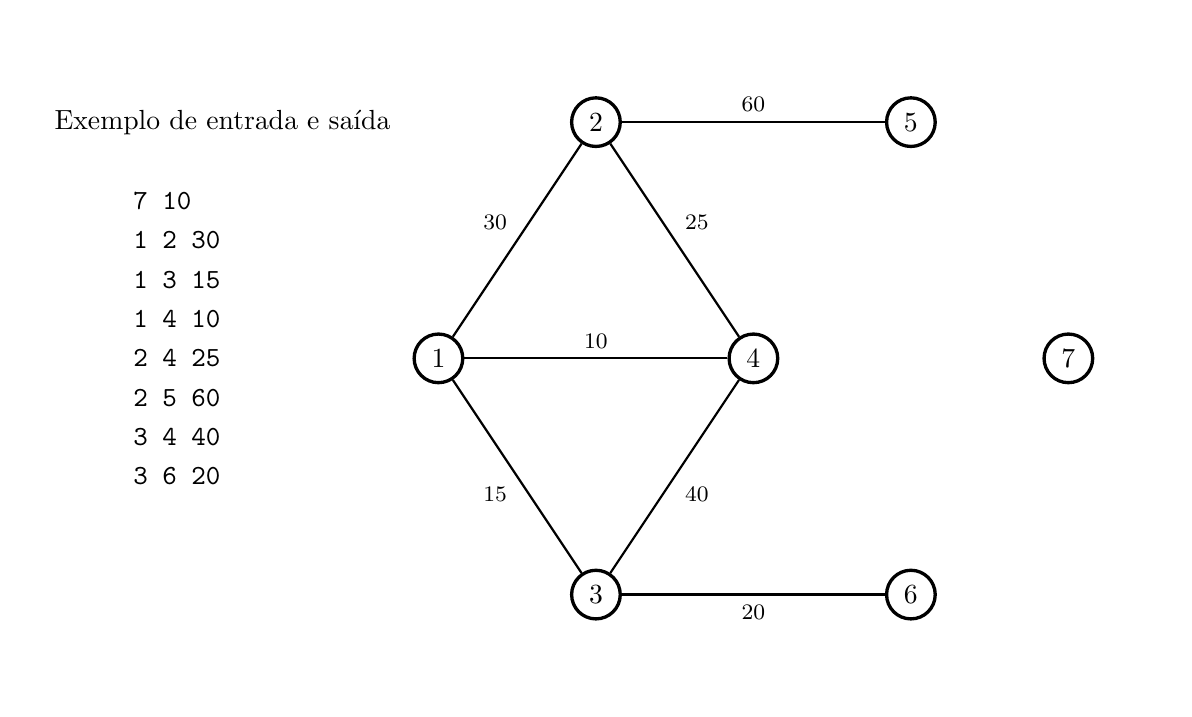
\begin{tikzpicture}
\node[draw,opacity=0] at (0, 0) {x};
\node[draw,opacity=0] at (14, 8) {x};

	\node[anchor=west] (header) at (0, 7.0) { \bbbold{Exemplo de entrada e saída} };


	\node[anchor=west] (line1) at (1.0, 6.0) { \bbtext{\texttt{7 10} } };







	\node[draw,circle,very thick] (node1) at (5.0, 4.0) { \bbtext{1} };

	\node[draw,circle,very thick] (node2) at (7.0, 7.0) { \bbtext{2} };

	\node[draw,circle,very thick] (node3) at (7.0, 1.0) { \bbtext{3} };

	\node[draw,circle,very thick] (node4) at (9.0, 4.0) { \bbtext{4} };

	\node[draw,circle,very thick] (node5) at (11.0, 7.0) { \bbtext{5} };

	\node[draw,circle,very thick] (node6) at (11.0, 1.0) { \bbtext{6} };

	\node[draw,circle,very thick] (node7) at (13.0, 4.0) { \bbtext{7} };


	\node[anchor=west] (line2) at (1.0, 5.5) { \bbtext{\texttt{1 2 30} } };








	\draw[thick](node1) to node[above left] { \footnotesize \bbinfo{30} } (node2);


	\node[anchor=west] (line3) at (1.0, 5.0) { \bbtext{\texttt{1 3 15} } };


	\draw[thick](node1) to node[below left] { \footnotesize \bbinfo{15} } (node3);


	\node[anchor=west] (line4) at (1.0, 4.5) { \bbtext{\texttt{1 4 10} } };


	\draw[thick](node1) to node[above] { \footnotesize \bbinfo{10} } (node4);


	\node[anchor=west] (line5) at (1.0, 4.0) { \bbtext{\texttt{2 4 25} } };


	\draw[thick](node2) to node[above right] { \footnotesize \bbinfo{25} } (node4);


	\node[anchor=west] (line6) at (1.0, 3.5) { \bbtext{\texttt{2 5 60} } };


	\draw[thick](node2) to node[above] { \footnotesize \bbinfo{60} } (node5);


	\node[anchor=west] (line7) at (1.0, 3.0) { \bbtext{\texttt{3 4 40} } };


	\draw[thick](node3) to node[below right] { \footnotesize \bbinfo{40} } (node4);


	\node[anchor=west] (line8) at (1.0, 2.5) { \bbtext{\texttt{3 6 20} } };


	\draw[thick](node3) to node[below] { \footnotesize \bbinfo{20} } (node6);

\end{tikzpicture}
\end{frame}
\begin{frame}[plain,t]
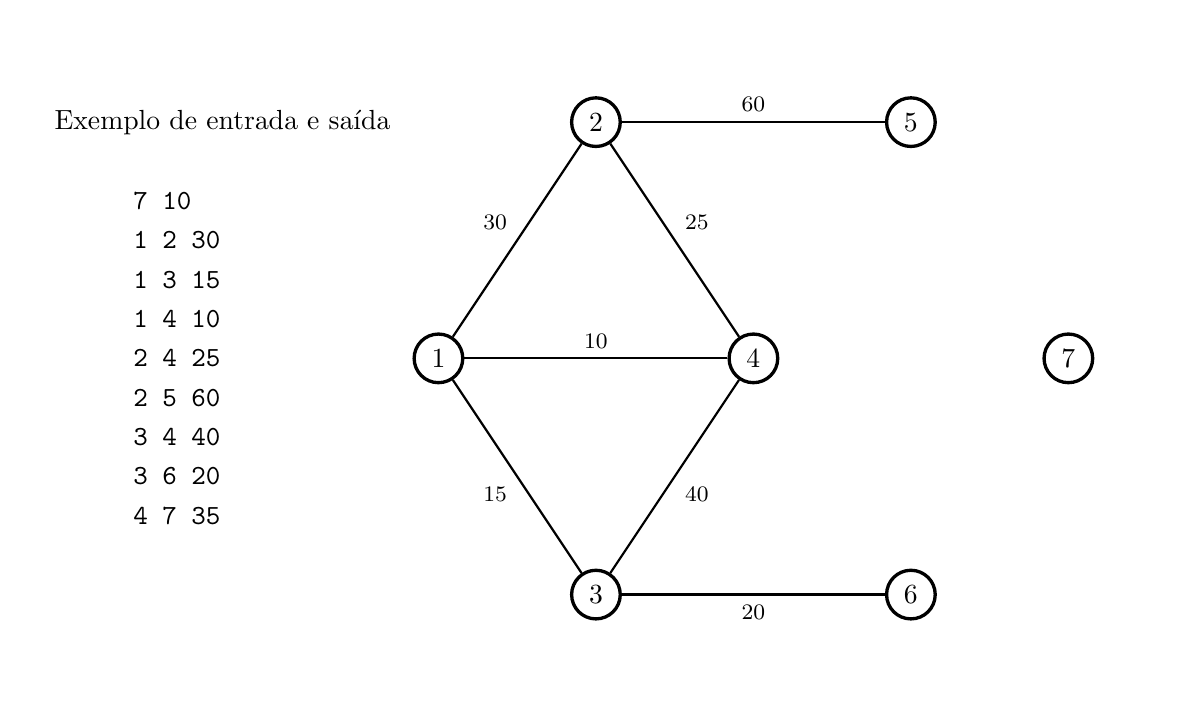
\begin{tikzpicture}
\node[draw,opacity=0] at (0, 0) {x};
\node[draw,opacity=0] at (14, 8) {x};

	\node[anchor=west] (header) at (0, 7.0) { \bbbold{Exemplo de entrada e saída} };


	\node[anchor=west] (line1) at (1.0, 6.0) { \bbtext{\texttt{7 10} } };







	\node[draw,circle,very thick] (node1) at (5.0, 4.0) { \bbtext{1} };

	\node[draw,circle,very thick] (node2) at (7.0, 7.0) { \bbtext{2} };

	\node[draw,circle,very thick] (node3) at (7.0, 1.0) { \bbtext{3} };

	\node[draw,circle,very thick] (node4) at (9.0, 4.0) { \bbtext{4} };

	\node[draw,circle,very thick] (node5) at (11.0, 7.0) { \bbtext{5} };

	\node[draw,circle,very thick] (node6) at (11.0, 1.0) { \bbtext{6} };

	\node[draw,circle,very thick] (node7) at (13.0, 4.0) { \bbtext{7} };


	\node[anchor=west] (line2) at (1.0, 5.5) { \bbtext{\texttt{1 2 30} } };








	\draw[thick](node1) to node[above left] { \footnotesize \bbinfo{30} } (node2);


	\node[anchor=west] (line3) at (1.0, 5.0) { \bbtext{\texttt{1 3 15} } };


	\draw[thick](node1) to node[below left] { \footnotesize \bbinfo{15} } (node3);


	\node[anchor=west] (line4) at (1.0, 4.5) { \bbtext{\texttt{1 4 10} } };


	\draw[thick](node1) to node[above] { \footnotesize \bbinfo{10} } (node4);


	\node[anchor=west] (line5) at (1.0, 4.0) { \bbtext{\texttt{2 4 25} } };


	\draw[thick](node2) to node[above right] { \footnotesize \bbinfo{25} } (node4);


	\node[anchor=west] (line6) at (1.0, 3.5) { \bbtext{\texttt{2 5 60} } };


	\draw[thick](node2) to node[above] { \footnotesize \bbinfo{60} } (node5);


	\node[anchor=west] (line7) at (1.0, 3.0) { \bbtext{\texttt{3 4 40} } };


	\draw[thick](node3) to node[below right] { \footnotesize \bbinfo{40} } (node4);


	\node[anchor=west] (line8) at (1.0, 2.5) { \bbtext{\texttt{3 6 20} } };


	\draw[thick](node3) to node[below] { \footnotesize \bbinfo{20} } (node6);


	\node[anchor=west] (line9) at (1.0, 2.0) { \bbtext{\texttt{4 7 35} } };

\end{tikzpicture}
\end{frame}
\begin{frame}[plain,t]
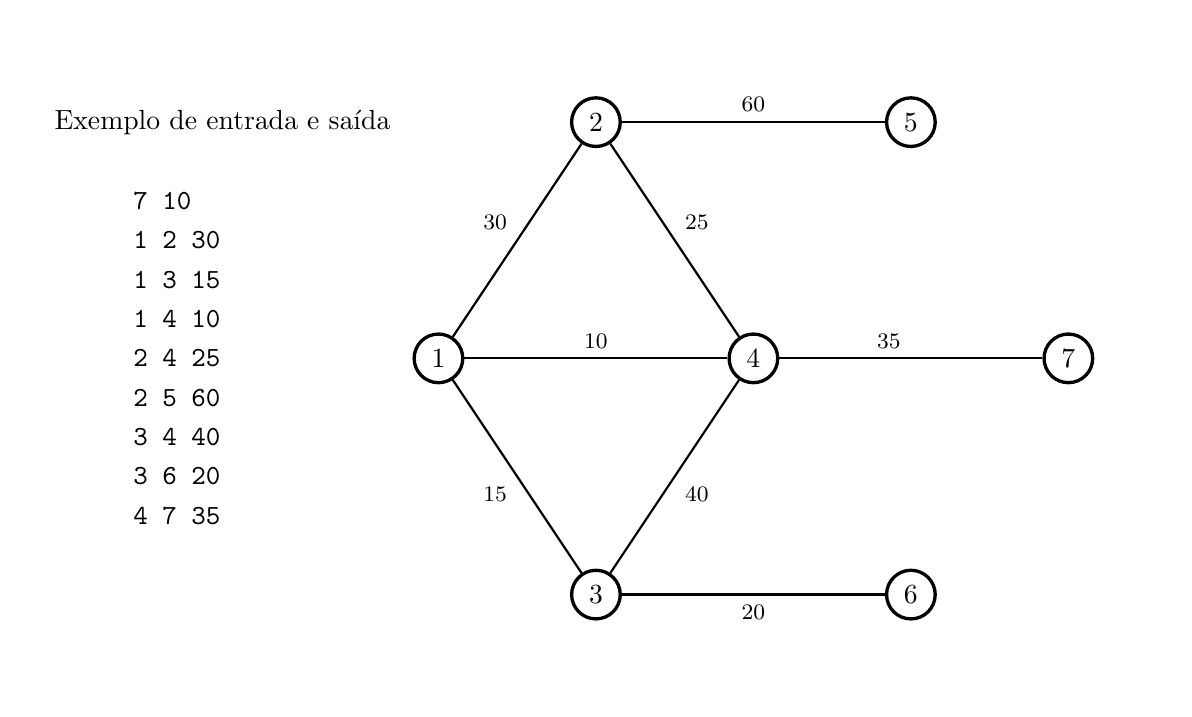
\begin{tikzpicture}
\node[draw,opacity=0] at (0, 0) {x};
\node[draw,opacity=0] at (14, 8) {x};

	\node[anchor=west] (header) at (0, 7.0) { \bbbold{Exemplo de entrada e saída} };


	\node[anchor=west] (line1) at (1.0, 6.0) { \bbtext{\texttt{7 10} } };







	\node[draw,circle,very thick] (node1) at (5.0, 4.0) { \bbtext{1} };

	\node[draw,circle,very thick] (node2) at (7.0, 7.0) { \bbtext{2} };

	\node[draw,circle,very thick] (node3) at (7.0, 1.0) { \bbtext{3} };

	\node[draw,circle,very thick] (node4) at (9.0, 4.0) { \bbtext{4} };

	\node[draw,circle,very thick] (node5) at (11.0, 7.0) { \bbtext{5} };

	\node[draw,circle,very thick] (node6) at (11.0, 1.0) { \bbtext{6} };

	\node[draw,circle,very thick] (node7) at (13.0, 4.0) { \bbtext{7} };


	\node[anchor=west] (line2) at (1.0, 5.5) { \bbtext{\texttt{1 2 30} } };








	\draw[thick](node1) to node[above left] { \footnotesize \bbinfo{30} } (node2);


	\node[anchor=west] (line3) at (1.0, 5.0) { \bbtext{\texttt{1 3 15} } };


	\draw[thick](node1) to node[below left] { \footnotesize \bbinfo{15} } (node3);


	\node[anchor=west] (line4) at (1.0, 4.5) { \bbtext{\texttt{1 4 10} } };


	\draw[thick](node1) to node[above] { \footnotesize \bbinfo{10} } (node4);


	\node[anchor=west] (line5) at (1.0, 4.0) { \bbtext{\texttt{2 4 25} } };


	\draw[thick](node2) to node[above right] { \footnotesize \bbinfo{25} } (node4);


	\node[anchor=west] (line6) at (1.0, 3.5) { \bbtext{\texttt{2 5 60} } };


	\draw[thick](node2) to node[above] { \footnotesize \bbinfo{60} } (node5);


	\node[anchor=west] (line7) at (1.0, 3.0) { \bbtext{\texttt{3 4 40} } };


	\draw[thick](node3) to node[below right] { \footnotesize \bbinfo{40} } (node4);


	\node[anchor=west] (line8) at (1.0, 2.5) { \bbtext{\texttt{3 6 20} } };


	\draw[thick](node3) to node[below] { \footnotesize \bbinfo{20} } (node6);


	\node[anchor=west] (line9) at (1.0, 2.0) { \bbtext{\texttt{4 7 35} } };


	\draw[thick](node4) to node[above left] { \footnotesize \bbinfo{35} } (node7);

\end{tikzpicture}
\end{frame}
\begin{frame}[plain,t]
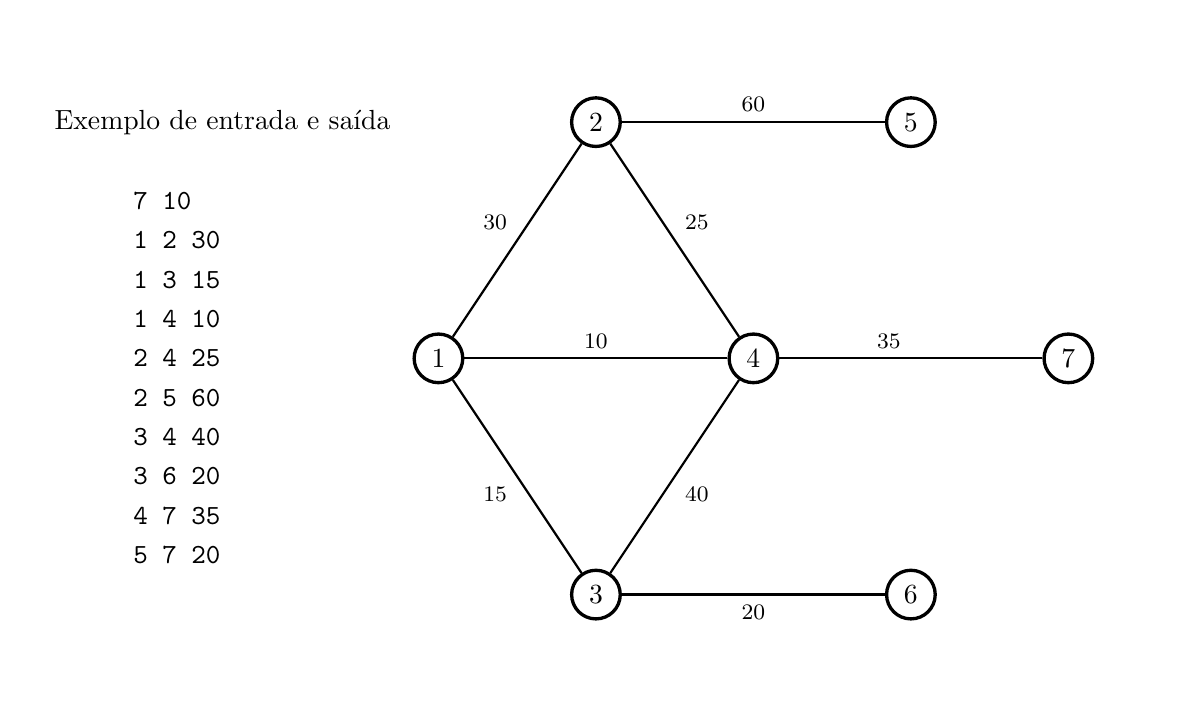
\begin{tikzpicture}
\node[draw,opacity=0] at (0, 0) {x};
\node[draw,opacity=0] at (14, 8) {x};

	\node[anchor=west] (header) at (0, 7.0) { \bbbold{Exemplo de entrada e saída} };


	\node[anchor=west] (line1) at (1.0, 6.0) { \bbtext{\texttt{7 10} } };







	\node[draw,circle,very thick] (node1) at (5.0, 4.0) { \bbtext{1} };

	\node[draw,circle,very thick] (node2) at (7.0, 7.0) { \bbtext{2} };

	\node[draw,circle,very thick] (node3) at (7.0, 1.0) { \bbtext{3} };

	\node[draw,circle,very thick] (node4) at (9.0, 4.0) { \bbtext{4} };

	\node[draw,circle,very thick] (node5) at (11.0, 7.0) { \bbtext{5} };

	\node[draw,circle,very thick] (node6) at (11.0, 1.0) { \bbtext{6} };

	\node[draw,circle,very thick] (node7) at (13.0, 4.0) { \bbtext{7} };


	\node[anchor=west] (line2) at (1.0, 5.5) { \bbtext{\texttt{1 2 30} } };








	\draw[thick](node1) to node[above left] { \footnotesize \bbinfo{30} } (node2);


	\node[anchor=west] (line3) at (1.0, 5.0) { \bbtext{\texttt{1 3 15} } };


	\draw[thick](node1) to node[below left] { \footnotesize \bbinfo{15} } (node3);


	\node[anchor=west] (line4) at (1.0, 4.5) { \bbtext{\texttt{1 4 10} } };


	\draw[thick](node1) to node[above] { \footnotesize \bbinfo{10} } (node4);


	\node[anchor=west] (line5) at (1.0, 4.0) { \bbtext{\texttt{2 4 25} } };


	\draw[thick](node2) to node[above right] { \footnotesize \bbinfo{25} } (node4);


	\node[anchor=west] (line6) at (1.0, 3.5) { \bbtext{\texttt{2 5 60} } };


	\draw[thick](node2) to node[above] { \footnotesize \bbinfo{60} } (node5);


	\node[anchor=west] (line7) at (1.0, 3.0) { \bbtext{\texttt{3 4 40} } };


	\draw[thick](node3) to node[below right] { \footnotesize \bbinfo{40} } (node4);


	\node[anchor=west] (line8) at (1.0, 2.5) { \bbtext{\texttt{3 6 20} } };


	\draw[thick](node3) to node[below] { \footnotesize \bbinfo{20} } (node6);


	\node[anchor=west] (line9) at (1.0, 2.0) { \bbtext{\texttt{4 7 35} } };


	\draw[thick](node4) to node[above left] { \footnotesize \bbinfo{35} } (node7);


	\node[anchor=west] (line10) at (1.0, 1.5) { \bbtext{\texttt{5 7 20} } };
\end{tikzpicture}
\end{frame}
\begin{frame}[plain,t]
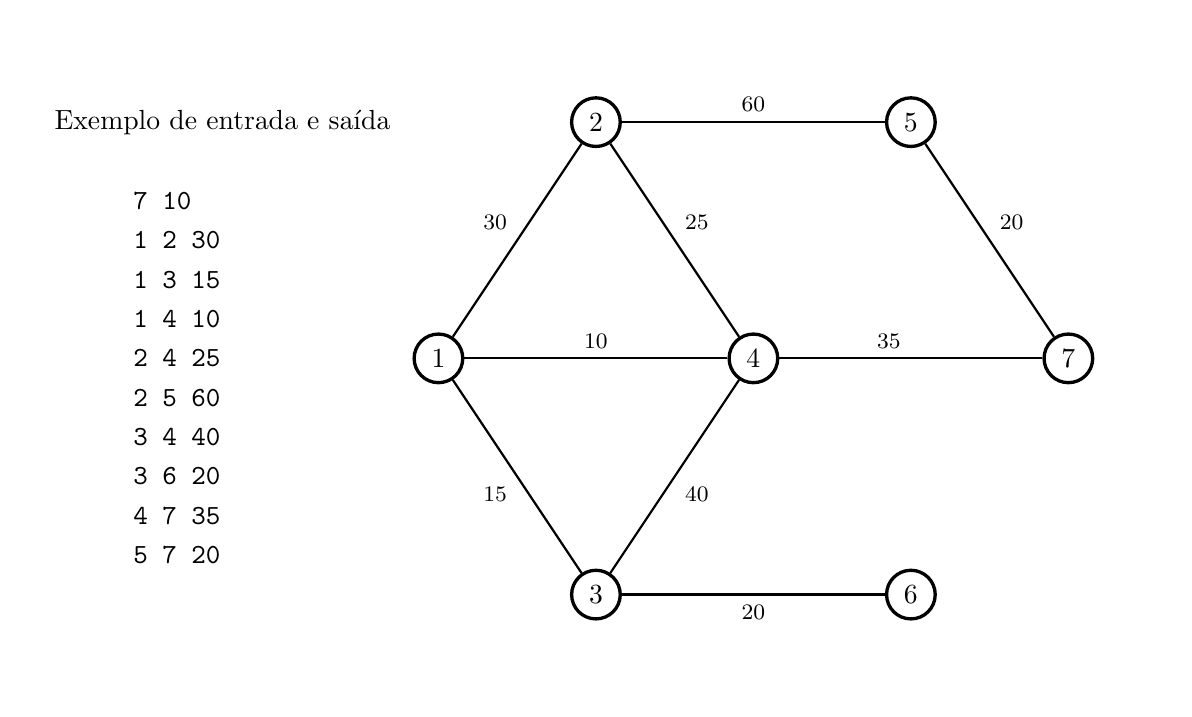
\begin{tikzpicture}
\node[draw,opacity=0] at (0, 0) {x};
\node[draw,opacity=0] at (14, 8) {x};

	\node[anchor=west] (header) at (0, 7.0) { \bbbold{Exemplo de entrada e saída} };


	\node[anchor=west] (line1) at (1.0, 6.0) { \bbtext{\texttt{7 10} } };







	\node[draw,circle,very thick] (node1) at (5.0, 4.0) { \bbtext{1} };

	\node[draw,circle,very thick] (node2) at (7.0, 7.0) { \bbtext{2} };

	\node[draw,circle,very thick] (node3) at (7.0, 1.0) { \bbtext{3} };

	\node[draw,circle,very thick] (node4) at (9.0, 4.0) { \bbtext{4} };

	\node[draw,circle,very thick] (node5) at (11.0, 7.0) { \bbtext{5} };

	\node[draw,circle,very thick] (node6) at (11.0, 1.0) { \bbtext{6} };

	\node[draw,circle,very thick] (node7) at (13.0, 4.0) { \bbtext{7} };


	\node[anchor=west] (line2) at (1.0, 5.5) { \bbtext{\texttt{1 2 30} } };








	\draw[thick](node1) to node[above left] { \footnotesize \bbinfo{30} } (node2);


	\node[anchor=west] (line3) at (1.0, 5.0) { \bbtext{\texttt{1 3 15} } };


	\draw[thick](node1) to node[below left] { \footnotesize \bbinfo{15} } (node3);


	\node[anchor=west] (line4) at (1.0, 4.5) { \bbtext{\texttt{1 4 10} } };


	\draw[thick](node1) to node[above] { \footnotesize \bbinfo{10} } (node4);


	\node[anchor=west] (line5) at (1.0, 4.0) { \bbtext{\texttt{2 4 25} } };


	\draw[thick](node2) to node[above right] { \footnotesize \bbinfo{25} } (node4);


	\node[anchor=west] (line6) at (1.0, 3.5) { \bbtext{\texttt{2 5 60} } };


	\draw[thick](node2) to node[above] { \footnotesize \bbinfo{60} } (node5);


	\node[anchor=west] (line7) at (1.0, 3.0) { \bbtext{\texttt{3 4 40} } };


	\draw[thick](node3) to node[below right] { \footnotesize \bbinfo{40} } (node4);


	\node[anchor=west] (line8) at (1.0, 2.5) { \bbtext{\texttt{3 6 20} } };


	\draw[thick](node3) to node[below] { \footnotesize \bbinfo{20} } (node6);


	\node[anchor=west] (line9) at (1.0, 2.0) { \bbtext{\texttt{4 7 35} } };


	\draw[thick](node4) to node[above left] { \footnotesize \bbinfo{35} } (node7);


	\node[anchor=west] (line10) at (1.0, 1.5) { \bbtext{\texttt{5 7 20} } };


	\draw[thick](node5) to node[above right] { \footnotesize \bbinfo{20} } (node7);

\end{tikzpicture}
\end{frame}
\begin{frame}[plain,t]
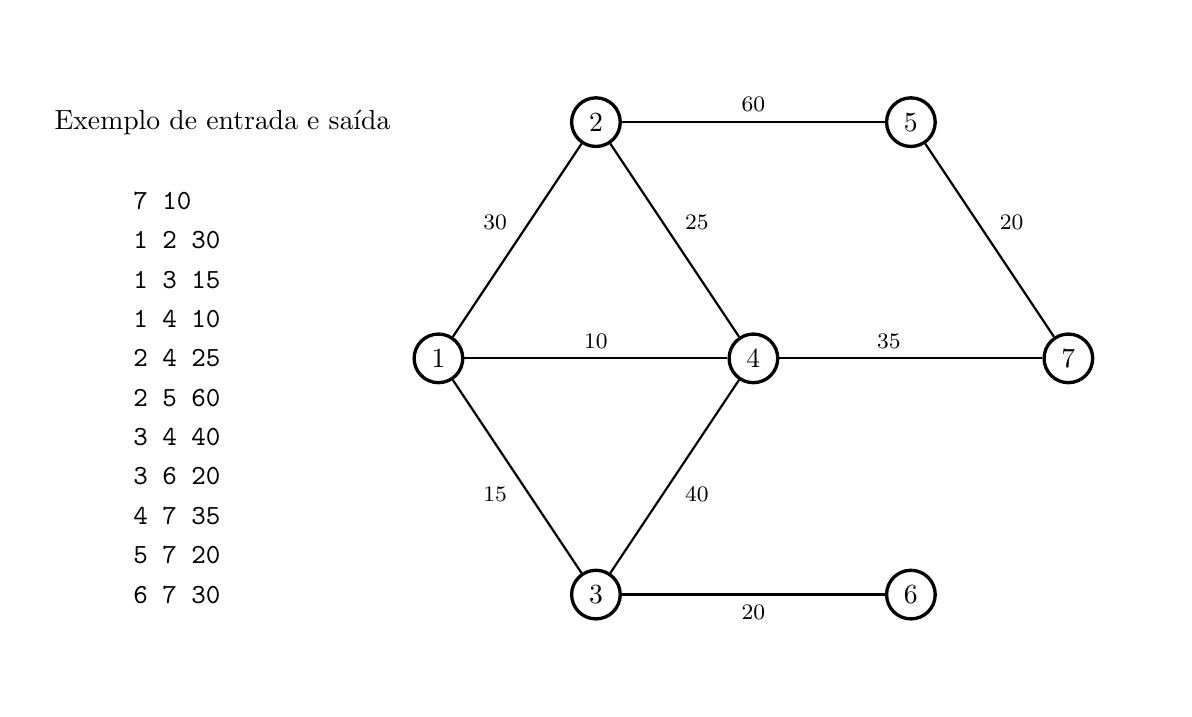
\begin{tikzpicture}
\node[draw,opacity=0] at (0, 0) {x};
\node[draw,opacity=0] at (14, 8) {x};

	\node[anchor=west] (header) at (0, 7.0) { \bbbold{Exemplo de entrada e saída} };


	\node[anchor=west] (line1) at (1.0, 6.0) { \bbtext{\texttt{7 10} } };







	\node[draw,circle,very thick] (node1) at (5.0, 4.0) { \bbtext{1} };

	\node[draw,circle,very thick] (node2) at (7.0, 7.0) { \bbtext{2} };

	\node[draw,circle,very thick] (node3) at (7.0, 1.0) { \bbtext{3} };

	\node[draw,circle,very thick] (node4) at (9.0, 4.0) { \bbtext{4} };

	\node[draw,circle,very thick] (node5) at (11.0, 7.0) { \bbtext{5} };

	\node[draw,circle,very thick] (node6) at (11.0, 1.0) { \bbtext{6} };

	\node[draw,circle,very thick] (node7) at (13.0, 4.0) { \bbtext{7} };


	\node[anchor=west] (line2) at (1.0, 5.5) { \bbtext{\texttt{1 2 30} } };








	\draw[thick](node1) to node[above left] { \footnotesize \bbinfo{30} } (node2);


	\node[anchor=west] (line3) at (1.0, 5.0) { \bbtext{\texttt{1 3 15} } };


	\draw[thick](node1) to node[below left] { \footnotesize \bbinfo{15} } (node3);


	\node[anchor=west] (line4) at (1.0, 4.5) { \bbtext{\texttt{1 4 10} } };


	\draw[thick](node1) to node[above] { \footnotesize \bbinfo{10} } (node4);


	\node[anchor=west] (line5) at (1.0, 4.0) { \bbtext{\texttt{2 4 25} } };


	\draw[thick](node2) to node[above right] { \footnotesize \bbinfo{25} } (node4);


	\node[anchor=west] (line6) at (1.0, 3.5) { \bbtext{\texttt{2 5 60} } };


	\draw[thick](node2) to node[above] { \footnotesize \bbinfo{60} } (node5);


	\node[anchor=west] (line7) at (1.0, 3.0) { \bbtext{\texttt{3 4 40} } };


	\draw[thick](node3) to node[below right] { \footnotesize \bbinfo{40} } (node4);


	\node[anchor=west] (line8) at (1.0, 2.5) { \bbtext{\texttt{3 6 20} } };


	\draw[thick](node3) to node[below] { \footnotesize \bbinfo{20} } (node6);


	\node[anchor=west] (line9) at (1.0, 2.0) { \bbtext{\texttt{4 7 35} } };


	\draw[thick](node4) to node[above left] { \footnotesize \bbinfo{35} } (node7);


	\node[anchor=west] (line10) at (1.0, 1.5) { \bbtext{\texttt{5 7 20} } };


	\draw[thick](node5) to node[above right] { \footnotesize \bbinfo{20} } (node7);


	\node[anchor=west] (line11) at (1.0, 1.0) { \bbtext{\texttt{6 7 30} } };
\end{tikzpicture}
\end{frame}
\begin{frame}[plain,t]
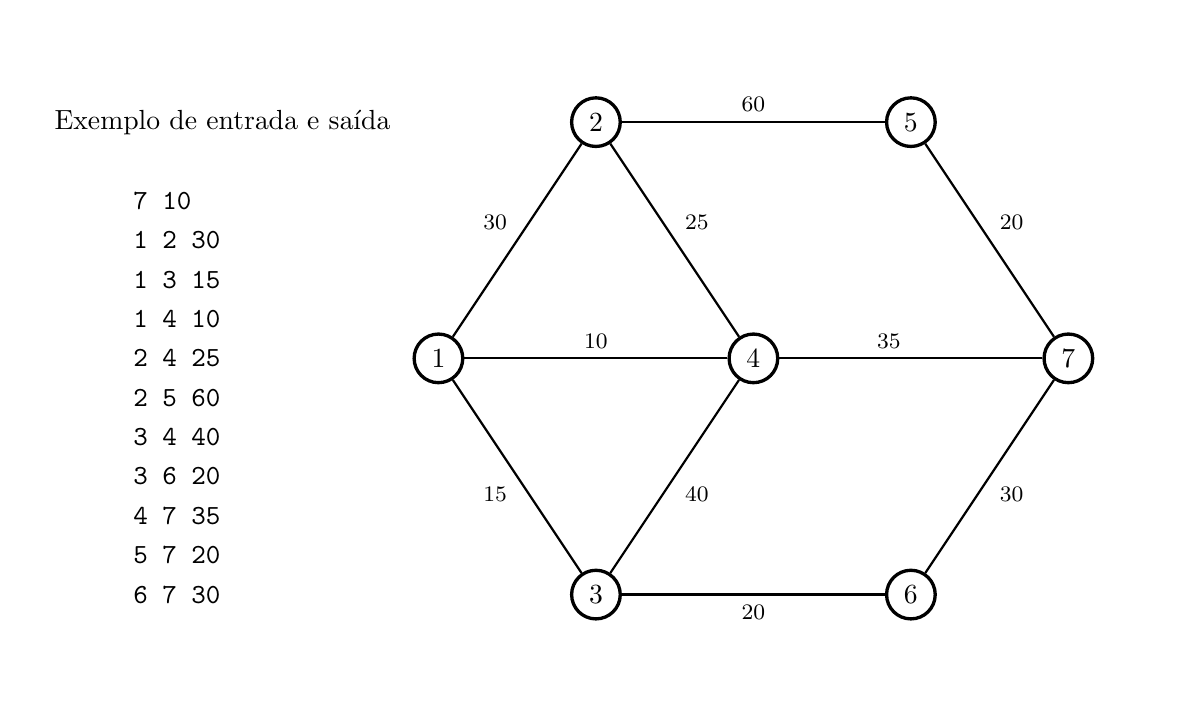
\begin{tikzpicture}
\node[draw,opacity=0] at (0, 0) {x};
\node[draw,opacity=0] at (14, 8) {x};

	\node[anchor=west] (header) at (0, 7.0) { \bbbold{Exemplo de entrada e saída} };


	\node[anchor=west] (line1) at (1.0, 6.0) { \bbtext{\texttt{7 10} } };







	\node[draw,circle,very thick] (node1) at (5.0, 4.0) { \bbtext{1} };

	\node[draw,circle,very thick] (node2) at (7.0, 7.0) { \bbtext{2} };

	\node[draw,circle,very thick] (node3) at (7.0, 1.0) { \bbtext{3} };

	\node[draw,circle,very thick] (node4) at (9.0, 4.0) { \bbtext{4} };

	\node[draw,circle,very thick] (node5) at (11.0, 7.0) { \bbtext{5} };

	\node[draw,circle,very thick] (node6) at (11.0, 1.0) { \bbtext{6} };

	\node[draw,circle,very thick] (node7) at (13.0, 4.0) { \bbtext{7} };


	\node[anchor=west] (line2) at (1.0, 5.5) { \bbtext{\texttt{1 2 30} } };








	\draw[thick](node1) to node[above left] { \footnotesize \bbinfo{30} } (node2);


	\node[anchor=west] (line3) at (1.0, 5.0) { \bbtext{\texttt{1 3 15} } };


	\draw[thick](node1) to node[below left] { \footnotesize \bbinfo{15} } (node3);


	\node[anchor=west] (line4) at (1.0, 4.5) { \bbtext{\texttt{1 4 10} } };


	\draw[thick](node1) to node[above] { \footnotesize \bbinfo{10} } (node4);


	\node[anchor=west] (line5) at (1.0, 4.0) { \bbtext{\texttt{2 4 25} } };


	\draw[thick](node2) to node[above right] { \footnotesize \bbinfo{25} } (node4);


	\node[anchor=west] (line6) at (1.0, 3.5) { \bbtext{\texttt{2 5 60} } };


	\draw[thick](node2) to node[above] { \footnotesize \bbinfo{60} } (node5);


	\node[anchor=west] (line7) at (1.0, 3.0) { \bbtext{\texttt{3 4 40} } };


	\draw[thick](node3) to node[below right] { \footnotesize \bbinfo{40} } (node4);


	\node[anchor=west] (line8) at (1.0, 2.5) { \bbtext{\texttt{3 6 20} } };


	\draw[thick](node3) to node[below] { \footnotesize \bbinfo{20} } (node6);


	\node[anchor=west] (line9) at (1.0, 2.0) { \bbtext{\texttt{4 7 35} } };


	\draw[thick](node4) to node[above left] { \footnotesize \bbinfo{35} } (node7);


	\node[anchor=west] (line10) at (1.0, 1.5) { \bbtext{\texttt{5 7 20} } };


	\draw[thick](node5) to node[above right] { \footnotesize \bbinfo{20} } (node7);


	\node[anchor=west] (line11) at (1.0, 1.0) { \bbtext{\texttt{6 7 30} } };

	\draw[thick](node6) to node[below right] { \footnotesize \bbinfo{30} } (node7);

\end{tikzpicture}
\end{frame}
\begin{frame}[plain,t]
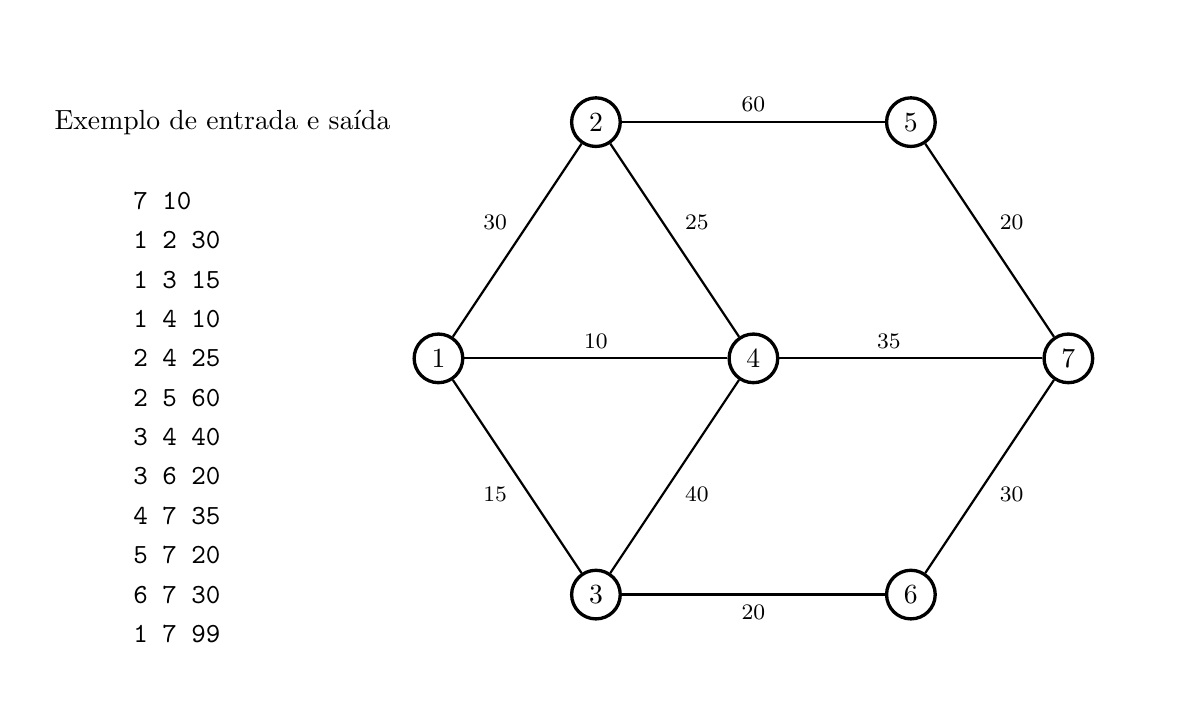
\begin{tikzpicture}
\node[draw,opacity=0] at (0, 0) {x};
\node[draw,opacity=0] at (14, 8) {x};

	\node[anchor=west] (header) at (0, 7.0) { \bbbold{Exemplo de entrada e saída} };


	\node[anchor=west] (line1) at (1.0, 6.0) { \bbtext{\texttt{7 10} } };







	\node[draw,circle,very thick] (node1) at (5.0, 4.0) { \bbtext{1} };

	\node[draw,circle,very thick] (node2) at (7.0, 7.0) { \bbtext{2} };

	\node[draw,circle,very thick] (node3) at (7.0, 1.0) { \bbtext{3} };

	\node[draw,circle,very thick] (node4) at (9.0, 4.0) { \bbtext{4} };

	\node[draw,circle,very thick] (node5) at (11.0, 7.0) { \bbtext{5} };

	\node[draw,circle,very thick] (node6) at (11.0, 1.0) { \bbtext{6} };

	\node[draw,circle,very thick] (node7) at (13.0, 4.0) { \bbtext{7} };


	\node[anchor=west] (line2) at (1.0, 5.5) { \bbtext{\texttt{1 2 30} } };








	\draw[thick](node1) to node[above left] { \footnotesize \bbinfo{30} } (node2);


	\node[anchor=west] (line3) at (1.0, 5.0) { \bbtext{\texttt{1 3 15} } };


	\draw[thick](node1) to node[below left] { \footnotesize \bbinfo{15} } (node3);


	\node[anchor=west] (line4) at (1.0, 4.5) { \bbtext{\texttt{1 4 10} } };


	\draw[thick](node1) to node[above] { \footnotesize \bbinfo{10} } (node4);


	\node[anchor=west] (line5) at (1.0, 4.0) { \bbtext{\texttt{2 4 25} } };


	\draw[thick](node2) to node[above right] { \footnotesize \bbinfo{25} } (node4);


	\node[anchor=west] (line6) at (1.0, 3.5) { \bbtext{\texttt{2 5 60} } };


	\draw[thick](node2) to node[above] { \footnotesize \bbinfo{60} } (node5);


	\node[anchor=west] (line7) at (1.0, 3.0) { \bbtext{\texttt{3 4 40} } };


	\draw[thick](node3) to node[below right] { \footnotesize \bbinfo{40} } (node4);


	\node[anchor=west] (line8) at (1.0, 2.5) { \bbtext{\texttt{3 6 20} } };


	\draw[thick](node3) to node[below] { \footnotesize \bbinfo{20} } (node6);


	\node[anchor=west] (line9) at (1.0, 2.0) { \bbtext{\texttt{4 7 35} } };


	\draw[thick](node4) to node[above left] { \footnotesize \bbinfo{35} } (node7);


	\node[anchor=west] (line10) at (1.0, 1.5) { \bbtext{\texttt{5 7 20} } };


	\draw[thick](node5) to node[above right] { \footnotesize \bbinfo{20} } (node7);


	\node[anchor=west] (line11) at (1.0, 1.0) { \bbtext{\texttt{6 7 30} } };

	\draw[thick](node6) to node[below right] { \footnotesize \bbinfo{30} } (node7);


	\node[anchor=west] (line12) at (1.0, 0.5) { \bbtext{\texttt{1 7 99} } };
\end{tikzpicture}
\end{frame}
\begin{frame}[plain,t]
\begin{tikzpicture}
\node[draw,opacity=0] at (0, 0) {x};
\node[draw,opacity=0] at (14, 8) {x};

	\node[anchor=west] (header) at (0, 7.0) { \bbbold{Exemplo de entrada e saída} };


	\node[anchor=west] (line1) at (1.0, 6.0) { \bbtext{\texttt{7 10} } };



	\node[anchor=west] (r) at (3.0, 0.0) { \footnotesize \bbcomment{ponto de partida} };




	\node[draw,circle,very thick] (node1) at (5.0, 4.0) { \bbtext{1} };

	\node[draw,circle,very thick] (node2) at (7.0, 7.0) { \bbtext{2} };

	\node[draw,circle,very thick] (node3) at (7.0, 1.0) { \bbtext{3} };

	\node[draw,circle,very thick] (node4) at (9.0, 4.0) { \bbtext{4} };

	\node[draw,circle,very thick] (node5) at (11.0, 7.0) { \bbtext{5} };

	\node[draw,circle,very thick] (node6) at (11.0, 1.0) { \bbtext{6} };

	\node[draw,circle,very thick] (node7) at (13.0, 4.0) { \bbtext{7} };


	\node[anchor=west] (line2) at (1.0, 5.5) { \bbtext{\texttt{1 2 30} } };








	\draw[thick](node1) to node[above left] { \footnotesize \bbinfo{30} } (node2);


	\node[anchor=west] (line3) at (1.0, 5.0) { \bbtext{\texttt{1 3 15} } };


	\draw[thick](node1) to node[below left] { \footnotesize \bbinfo{15} } (node3);


	\node[anchor=west] (line4) at (1.0, 4.5) { \bbtext{\texttt{1 4 10} } };


	\draw[thick](node1) to node[above] { \footnotesize \bbinfo{10} } (node4);


	\node[anchor=west] (line5) at (1.0, 4.0) { \bbtext{\texttt{2 4 25} } };


	\draw[thick](node2) to node[above right] { \footnotesize \bbinfo{25} } (node4);


	\node[anchor=west] (line6) at (1.0, 3.5) { \bbtext{\texttt{2 5 60} } };


	\draw[thick](node2) to node[above] { \footnotesize \bbinfo{60} } (node5);


	\node[anchor=west] (line7) at (1.0, 3.0) { \bbtext{\texttt{3 4 40} } };


	\draw[thick](node3) to node[below right] { \footnotesize \bbinfo{40} } (node4);


	\node[anchor=west] (line8) at (1.0, 2.5) { \bbtext{\texttt{3 6 20} } };


	\draw[thick](node3) to node[below] { \footnotesize \bbinfo{20} } (node6);


	\node[anchor=west] (line9) at (1.0, 2.0) { \bbtext{\texttt{4 7 35} } };


	\draw[thick](node4) to node[above left] { \footnotesize \bbinfo{35} } (node7);


	\node[anchor=west] (line10) at (1.0, 1.5) { \bbtext{\texttt{5 7 20} } };


	\draw[thick](node5) to node[above right] { \footnotesize \bbinfo{20} } (node7);


	\node[anchor=west] (line11) at (1.0, 1.0) { \bbtext{\texttt{6 7 30} } };

	\draw[thick](node6) to node[below right] { \footnotesize \bbinfo{30} } (node7);


	\node[anchor=west] (line12) at (1.0, 0.5) { \bbtext{\texttt{1 7 99} } };

	\draw[color=BBViolet,-latex] (1.25, 0.25) to (1.25, 0) to (3, 0);;


\end{tikzpicture}
\end{frame}
\begin{frame}[plain,t]
\begin{tikzpicture}
\node[draw,opacity=0] at (0, 0) {x};
\node[draw,opacity=0] at (14, 8) {x};

	\node[anchor=west] (header) at (0, 7.0) { \bbbold{Exemplo de entrada e saída} };


	\node[anchor=west] (line1) at (1.0, 6.0) { \bbtext{\texttt{7 10} } };



	\node[anchor=west] (r) at (3.0, 0.0) { \footnotesize \bbcomment{ponto de partida} };




	\node[draw,circle,very thick,fill=BBGreen] (node1) at (5.0, 4.0) { \bbtext{1} };

	\node[draw,circle,very thick] (node2) at (7.0, 7.0) { \bbtext{2} };

	\node[draw,circle,very thick] (node3) at (7.0, 1.0) { \bbtext{3} };

	\node[draw,circle,very thick] (node4) at (9.0, 4.0) { \bbtext{4} };

	\node[draw,circle,very thick] (node5) at (11.0, 7.0) { \bbtext{5} };

	\node[draw,circle,very thick] (node6) at (11.0, 1.0) { \bbtext{6} };

	\node[draw,circle,very thick] (node7) at (13.0, 4.0) { \bbtext{7} };


	\node[anchor=west] (line2) at (1.0, 5.5) { \bbtext{\texttt{1 2 30} } };








	\draw[thick](node1) to node[above left] { \footnotesize \bbinfo{30} } (node2);


	\node[anchor=west] (line3) at (1.0, 5.0) { \bbtext{\texttt{1 3 15} } };


	\draw[thick](node1) to node[below left] { \footnotesize \bbinfo{15} } (node3);


	\node[anchor=west] (line4) at (1.0, 4.5) { \bbtext{\texttt{1 4 10} } };


	\draw[thick](node1) to node[above] { \footnotesize \bbinfo{10} } (node4);


	\node[anchor=west] (line5) at (1.0, 4.0) { \bbtext{\texttt{2 4 25} } };


	\draw[thick](node2) to node[above right] { \footnotesize \bbinfo{25} } (node4);


	\node[anchor=west] (line6) at (1.0, 3.5) { \bbtext{\texttt{2 5 60} } };


	\draw[thick](node2) to node[above] { \footnotesize \bbinfo{60} } (node5);


	\node[anchor=west] (line7) at (1.0, 3.0) { \bbtext{\texttt{3 4 40} } };


	\draw[thick](node3) to node[below right] { \footnotesize \bbinfo{40} } (node4);


	\node[anchor=west] (line8) at (1.0, 2.5) { \bbtext{\texttt{3 6 20} } };


	\draw[thick](node3) to node[below] { \footnotesize \bbinfo{20} } (node6);


	\node[anchor=west] (line9) at (1.0, 2.0) { \bbtext{\texttt{4 7 35} } };


	\draw[thick](node4) to node[above left] { \footnotesize \bbinfo{35} } (node7);


	\node[anchor=west] (line10) at (1.0, 1.5) { \bbtext{\texttt{5 7 20} } };


	\draw[thick](node5) to node[above right] { \footnotesize \bbinfo{20} } (node7);


	\node[anchor=west] (line11) at (1.0, 1.0) { \bbtext{\texttt{6 7 30} } };

	\draw[thick](node6) to node[below right] { \footnotesize \bbinfo{30} } (node7);


	\node[anchor=west] (line12) at (1.0, 0.5) { \bbtext{\texttt{1 7 99} } };

	\draw[color=BBViolet,-latex] (1.25, 0.25) to (1.25, 0) to (3, 0);;



\end{tikzpicture}
\end{frame}
\begin{frame}[plain,t]
\begin{tikzpicture}
\node[draw,opacity=0] at (0, 0) {x};
\node[draw,opacity=0] at (14, 8) {x};

	\node[anchor=west] (header) at (0, 7.0) { \bbbold{Exemplo de entrada e saída} };


	\node[anchor=west] (line1) at (1.0, 6.0) { \bbtext{\texttt{7 10} } };



	\node[anchor=west] (r) at (3.0, 0.0) { \footnotesize \bbcomment{destino} };




	\node[draw,circle,very thick,fill=BBGreen] (node1) at (5.0, 4.0) { \bbtext{1} };

	\node[draw,circle,very thick] (node2) at (7.0, 7.0) { \bbtext{2} };

	\node[draw,circle,very thick] (node3) at (7.0, 1.0) { \bbtext{3} };

	\node[draw,circle,very thick] (node4) at (9.0, 4.0) { \bbtext{4} };

	\node[draw,circle,very thick] (node5) at (11.0, 7.0) { \bbtext{5} };

	\node[draw,circle,very thick] (node6) at (11.0, 1.0) { \bbtext{6} };

	\node[draw,circle,very thick] (node7) at (13.0, 4.0) { \bbtext{7} };


	\node[anchor=west] (line2) at (1.0, 5.5) { \bbtext{\texttt{1 2 30} } };








	\draw[thick](node1) to node[above left] { \footnotesize \bbinfo{30} } (node2);


	\node[anchor=west] (line3) at (1.0, 5.0) { \bbtext{\texttt{1 3 15} } };


	\draw[thick](node1) to node[below left] { \footnotesize \bbinfo{15} } (node3);


	\node[anchor=west] (line4) at (1.0, 4.5) { \bbtext{\texttt{1 4 10} } };


	\draw[thick](node1) to node[above] { \footnotesize \bbinfo{10} } (node4);


	\node[anchor=west] (line5) at (1.0, 4.0) { \bbtext{\texttt{2 4 25} } };


	\draw[thick](node2) to node[above right] { \footnotesize \bbinfo{25} } (node4);


	\node[anchor=west] (line6) at (1.0, 3.5) { \bbtext{\texttt{2 5 60} } };


	\draw[thick](node2) to node[above] { \footnotesize \bbinfo{60} } (node5);


	\node[anchor=west] (line7) at (1.0, 3.0) { \bbtext{\texttt{3 4 40} } };


	\draw[thick](node3) to node[below right] { \footnotesize \bbinfo{40} } (node4);


	\node[anchor=west] (line8) at (1.0, 2.5) { \bbtext{\texttt{3 6 20} } };


	\draw[thick](node3) to node[below] { \footnotesize \bbinfo{20} } (node6);


	\node[anchor=west] (line9) at (1.0, 2.0) { \bbtext{\texttt{4 7 35} } };


	\draw[thick](node4) to node[above left] { \footnotesize \bbinfo{35} } (node7);


	\node[anchor=west] (line10) at (1.0, 1.5) { \bbtext{\texttt{5 7 20} } };


	\draw[thick](node5) to node[above right] { \footnotesize \bbinfo{20} } (node7);


	\node[anchor=west] (line11) at (1.0, 1.0) { \bbtext{\texttt{6 7 30} } };

	\draw[thick](node6) to node[below right] { \footnotesize \bbinfo{30} } (node7);


	\node[anchor=west] (line12) at (1.0, 0.5) { \bbtext{\texttt{1 7 99} } };

	\draw[color=BBViolet,-latex] (1.65, 0.25) to (1.65, 0) to (3, 0);;




\end{tikzpicture}
\end{frame}
\begin{frame}[plain,t]
\begin{tikzpicture}
\node[draw,opacity=0] at (0, 0) {x};
\node[draw,opacity=0] at (14, 8) {x};

	\node[anchor=west] (header) at (0, 7.0) { \bbbold{Exemplo de entrada e saída} };


	\node[anchor=west] (line1) at (1.0, 6.0) { \bbtext{\texttt{7 10} } };



	\node[anchor=west] (r) at (3.0, 0.0) { \footnotesize \bbcomment{destino} };




	\node[draw,circle,very thick,fill=BBGreen] (node1) at (5.0, 4.0) { \bbtext{1} };

	\node[draw,circle,very thick] (node2) at (7.0, 7.0) { \bbtext{2} };

	\node[draw,circle,very thick] (node3) at (7.0, 1.0) { \bbtext{3} };

	\node[draw,circle,very thick] (node4) at (9.0, 4.0) { \bbtext{4} };

	\node[draw,circle,very thick] (node5) at (11.0, 7.0) { \bbtext{5} };

	\node[draw,circle,very thick] (node6) at (11.0, 1.0) { \bbtext{6} };

	\node[draw,circle,very thick,fill=BBCyan] (node7) at (13.0, 4.0) { \bbtext{7} };


	\node[anchor=west] (line2) at (1.0, 5.5) { \bbtext{\texttt{1 2 30} } };








	\draw[thick](node1) to node[above left] { \footnotesize \bbinfo{30} } (node2);


	\node[anchor=west] (line3) at (1.0, 5.0) { \bbtext{\texttt{1 3 15} } };


	\draw[thick](node1) to node[below left] { \footnotesize \bbinfo{15} } (node3);


	\node[anchor=west] (line4) at (1.0, 4.5) { \bbtext{\texttt{1 4 10} } };


	\draw[thick](node1) to node[above] { \footnotesize \bbinfo{10} } (node4);


	\node[anchor=west] (line5) at (1.0, 4.0) { \bbtext{\texttt{2 4 25} } };


	\draw[thick](node2) to node[above right] { \footnotesize \bbinfo{25} } (node4);


	\node[anchor=west] (line6) at (1.0, 3.5) { \bbtext{\texttt{2 5 60} } };


	\draw[thick](node2) to node[above] { \footnotesize \bbinfo{60} } (node5);


	\node[anchor=west] (line7) at (1.0, 3.0) { \bbtext{\texttt{3 4 40} } };


	\draw[thick](node3) to node[below right] { \footnotesize \bbinfo{40} } (node4);


	\node[anchor=west] (line8) at (1.0, 2.5) { \bbtext{\texttt{3 6 20} } };


	\draw[thick](node3) to node[below] { \footnotesize \bbinfo{20} } (node6);


	\node[anchor=west] (line9) at (1.0, 2.0) { \bbtext{\texttt{4 7 35} } };


	\draw[thick](node4) to node[above left] { \footnotesize \bbinfo{35} } (node7);


	\node[anchor=west] (line10) at (1.0, 1.5) { \bbtext{\texttt{5 7 20} } };


	\draw[thick](node5) to node[above right] { \footnotesize \bbinfo{20} } (node7);


	\node[anchor=west] (line11) at (1.0, 1.0) { \bbtext{\texttt{6 7 30} } };

	\draw[thick](node6) to node[below right] { \footnotesize \bbinfo{30} } (node7);


	\node[anchor=west] (line12) at (1.0, 0.5) { \bbtext{\texttt{1 7 99} } };

	\draw[color=BBViolet,-latex] (1.65, 0.25) to (1.65, 0) to (3, 0);;





\end{tikzpicture}
\end{frame}
\begin{frame}[plain,t]
\begin{tikzpicture}
\node[draw,opacity=0] at (0, 0) {x};
\node[draw,opacity=0] at (14, 8) {x};

	\node[anchor=west] (header) at (0, 7.0) { \bbbold{Exemplo de entrada e saída} };


	\node[anchor=west] (line1) at (1.0, 6.0) { \bbtext{\texttt{7 10} } };



	\node[anchor=west] (r) at (3.0, 0.0) { \footnotesize \bbcomment{\# de turistas} };




	\node[draw,circle,very thick,fill=BBGreen] (node1) at (5.0, 4.0) { \bbtext{1} };

	\node[draw,circle,very thick] (node2) at (7.0, 7.0) { \bbtext{2} };

	\node[draw,circle,very thick] (node3) at (7.0, 1.0) { \bbtext{3} };

	\node[draw,circle,very thick] (node4) at (9.0, 4.0) { \bbtext{4} };

	\node[draw,circle,very thick] (node5) at (11.0, 7.0) { \bbtext{5} };

	\node[draw,circle,very thick] (node6) at (11.0, 1.0) { \bbtext{6} };

	\node[draw,circle,very thick,fill=BBCyan] (node7) at (13.0, 4.0) { \bbtext{7} };


	\node[anchor=west] (line2) at (1.0, 5.5) { \bbtext{\texttt{1 2 30} } };








	\draw[thick](node1) to node[above left] { \footnotesize \bbinfo{30} } (node2);


	\node[anchor=west] (line3) at (1.0, 5.0) { \bbtext{\texttt{1 3 15} } };


	\draw[thick](node1) to node[below left] { \footnotesize \bbinfo{15} } (node3);


	\node[anchor=west] (line4) at (1.0, 4.5) { \bbtext{\texttt{1 4 10} } };


	\draw[thick](node1) to node[above] { \footnotesize \bbinfo{10} } (node4);


	\node[anchor=west] (line5) at (1.0, 4.0) { \bbtext{\texttt{2 4 25} } };


	\draw[thick](node2) to node[above right] { \footnotesize \bbinfo{25} } (node4);


	\node[anchor=west] (line6) at (1.0, 3.5) { \bbtext{\texttt{2 5 60} } };


	\draw[thick](node2) to node[above] { \footnotesize \bbinfo{60} } (node5);


	\node[anchor=west] (line7) at (1.0, 3.0) { \bbtext{\texttt{3 4 40} } };


	\draw[thick](node3) to node[below right] { \footnotesize \bbinfo{40} } (node4);


	\node[anchor=west] (line8) at (1.0, 2.5) { \bbtext{\texttt{3 6 20} } };


	\draw[thick](node3) to node[below] { \footnotesize \bbinfo{20} } (node6);


	\node[anchor=west] (line9) at (1.0, 2.0) { \bbtext{\texttt{4 7 35} } };


	\draw[thick](node4) to node[above left] { \footnotesize \bbinfo{35} } (node7);


	\node[anchor=west] (line10) at (1.0, 1.5) { \bbtext{\texttt{5 7 20} } };


	\draw[thick](node5) to node[above right] { \footnotesize \bbinfo{20} } (node7);


	\node[anchor=west] (line11) at (1.0, 1.0) { \bbtext{\texttt{6 7 30} } };

	\draw[thick](node6) to node[below right] { \footnotesize \bbinfo{30} } (node7);


	\node[anchor=west] (line12) at (1.0, 0.5) { \bbtext{\texttt{1 7 99} } };

	\draw[color=BBViolet,-latex] (2.15, 0.25) to (2.15, 0) to (3, 0);;






\end{tikzpicture}
\end{frame}
\begin{frame}[plain,t]
\begin{tikzpicture}
\node[draw,opacity=0] at (0, 0) {x};
\node[draw,opacity=0] at (14, 8) {x};

	\node[anchor=west] (header) at (0, 7.0) { \bbbold{Exemplo de entrada e saída} };


	\node[anchor=west] (line1) at (1.0, 6.0) { \bbtext{\texttt{7 10} } };







	\node[draw,circle,very thick,fill=BBGreen] (node1) at (5.0, 4.0) { \bbtext{1} };

	\node[draw,circle,very thick] (node2) at (7.0, 7.0) { \bbtext{2} };

	\node[draw,circle,very thick] (node3) at (7.0, 1.0) { \bbtext{3} };

	\node[draw,circle,very thick] (node4) at (9.0, 4.0) { \bbtext{4} };

	\node[draw,circle,very thick] (node5) at (11.0, 7.0) { \bbtext{5} };

	\node[draw,circle,very thick] (node6) at (11.0, 1.0) { \bbtext{6} };

	\node[draw,circle,very thick,fill=BBCyan] (node7) at (13.0, 4.0) { \bbtext{7} };


	\node[anchor=west] (line2) at (1.0, 5.5) { \bbtext{\texttt{1 2 30} } };








	\draw[thick,color=BBCyan,very thick,dashed](node1) to node[above left] { \footnotesize \bbinfo{30} } (node2);


	\node[anchor=west] (line3) at (1.0, 5.0) { \bbtext{\texttt{1 3 15} } };


	\draw[thick](node1) to node[below left] { \footnotesize \bbinfo{15} } (node3);


	\node[anchor=west] (line4) at (1.0, 4.5) { \bbtext{\texttt{1 4 10} } };


	\draw[thick](node1) to node[above] { \footnotesize \bbinfo{10} } (node4);


	\node[anchor=west] (line5) at (1.0, 4.0) { \bbtext{\texttt{2 4 25} } };


	\draw[thick,color=BBCyan,very thick,dashed](node2) to node[above right] { \footnotesize \bbinfo{25} } (node4);


	\node[anchor=west] (line6) at (1.0, 3.5) { \bbtext{\texttt{2 5 60} } };


	\draw[thick](node2) to node[above] { \footnotesize \bbinfo{60} } (node5);


	\node[anchor=west] (line7) at (1.0, 3.0) { \bbtext{\texttt{3 4 40} } };


	\draw[thick](node3) to node[below right] { \footnotesize \bbinfo{40} } (node4);


	\node[anchor=west] (line8) at (1.0, 2.5) { \bbtext{\texttt{3 6 20} } };


	\draw[thick](node3) to node[below] { \footnotesize \bbinfo{20} } (node6);


	\node[anchor=west] (line9) at (1.0, 2.0) { \bbtext{\texttt{4 7 35} } };


	\draw[thick,color=BBCyan,very thick,dashed](node4) to node[above left] { \footnotesize \bbinfo{35} } (node7);


	\node[anchor=west] (line10) at (1.0, 1.5) { \bbtext{\texttt{5 7 20} } };


	\draw[thick](node5) to node[above right] { \footnotesize \bbinfo{20} } (node7);


	\node[anchor=west] (line11) at (1.0, 1.0) { \bbtext{\texttt{6 7 30} } };

	\draw[thick](node6) to node[below right] { \footnotesize \bbinfo{30} } (node7);


	\node[anchor=west] (line12) at (1.0, 0.5) { \bbtext{\texttt{1 7 99} } };











\end{tikzpicture}
\end{frame}
\begin{frame}[plain,t]
\begin{tikzpicture}
\node[draw,opacity=0] at (0, 0) {x};
\node[draw,opacity=0] at (14, 8) {x};

	\node[anchor=west] (header) at (0, 7.0) { \bbbold{Exemplo de entrada e saída} };


	\node[anchor=west] (line1) at (1.0, 6.0) { \bbtext{\texttt{7 10} } };


	\draw[->,color=BBBlack,-latex,very thick] (2.5, 2.5) to  (3.5, 2.5);

	\node[anchor=west] (r) at (3.5, 2.5) { \bbinfo{5} };




	\node[draw,circle,very thick,fill=BBGreen] (node1) at (5.0, 4.0) { \bbtext{1} };

	\node[draw,circle,very thick] (node2) at (7.0, 7.0) { \bbtext{2} };

	\node[draw,circle,very thick] (node3) at (7.0, 1.0) { \bbtext{3} };

	\node[draw,circle,very thick] (node4) at (9.0, 4.0) { \bbtext{4} };

	\node[draw,circle,very thick] (node5) at (11.0, 7.0) { \bbtext{5} };

	\node[draw,circle,very thick] (node6) at (11.0, 1.0) { \bbtext{6} };

	\node[draw,circle,very thick,fill=BBCyan] (node7) at (13.0, 4.0) { \bbtext{7} };


	\node[anchor=west] (line2) at (1.0, 5.5) { \bbtext{\texttt{1 2 30} } };








	\draw[thick,color=BBCyan,very thick,dashed](node1) to node[above left] { \footnotesize \bbinfo{30} } (node2);


	\node[anchor=west] (line3) at (1.0, 5.0) { \bbtext{\texttt{1 3 15} } };


	\draw[thick](node1) to node[below left] { \footnotesize \bbinfo{15} } (node3);


	\node[anchor=west] (line4) at (1.0, 4.5) { \bbtext{\texttt{1 4 10} } };


	\draw[thick](node1) to node[above] { \footnotesize \bbinfo{10} } (node4);


	\node[anchor=west] (line5) at (1.0, 4.0) { \bbtext{\texttt{2 4 25} } };


	\draw[thick,color=BBCyan,very thick,dashed](node2) to node[above right] { \footnotesize \bbinfo{25} } (node4);


	\node[anchor=west] (line6) at (1.0, 3.5) { \bbtext{\texttt{2 5 60} } };


	\draw[thick](node2) to node[above] { \footnotesize \bbinfo{60} } (node5);


	\node[anchor=west] (line7) at (1.0, 3.0) { \bbtext{\texttt{3 4 40} } };


	\draw[thick](node3) to node[below right] { \footnotesize \bbinfo{40} } (node4);


	\node[anchor=west] (line8) at (1.0, 2.5) { \bbtext{\texttt{3 6 20} } };


	\draw[thick](node3) to node[below] { \footnotesize \bbinfo{20} } (node6);


	\node[anchor=west] (line9) at (1.0, 2.0) { \bbtext{\texttt{4 7 35} } };


	\draw[thick,color=BBCyan,very thick,dashed](node4) to node[above left] { \footnotesize \bbinfo{35} } (node7);


	\node[anchor=west] (line10) at (1.0, 1.5) { \bbtext{\texttt{5 7 20} } };


	\draw[thick](node5) to node[above right] { \footnotesize \bbinfo{20} } (node7);


	\node[anchor=west] (line11) at (1.0, 1.0) { \bbtext{\texttt{6 7 30} } };

	\draw[thick](node6) to node[below right] { \footnotesize \bbinfo{30} } (node7);


	\node[anchor=west] (line12) at (1.0, 0.5) { \bbtext{\texttt{1 7 99} } };














\end{tikzpicture}
\end{frame}
\begin{frame}[plain,t]
\begin{tikzpicture}
\node[draw,opacity=0] at (0, 0) {x};
\node[draw,opacity=0] at (14, 8) {x};

	\node[anchor=west] (header) at (0.0, 7.0) { \Large \bbbold{Solução} };

\end{tikzpicture}
\end{frame}
\end{document}
